\documentclass[10pt,a4paper,twoside,headinclude,footinclude,color]{./latex-notes-cls/edoars-notes}
\graphicspath{ {Immagini/} }

\hypersetup{pdfauthor={Edoardo Signorini},
            pdftitle={Crittografia a chiave pubblica},
            pdfcreator={Latex with hyperref}}

\begin{document}
%MATERIALE INIZIALE
\begin{frontespizio}
\Preambolo{\usepackage{iwona}}
\Universita{Roma Tre}
\Logo{Immagini/logo}
\Facolta{Matematica}
\Scuola{}
\Piede{A.A. 2016--2017, Semestre II}
\Titoletto{Appunti integrativi}
\Titolo{Crittografia a chiave pubblica}
\Sottotitolo{CR410}
\NCandidato{Di}
\Candidato{Edoardo Signorini}
\end{frontespizio}
\tableofcontents

%MATERIALE PRINCIPALE
%!TEX root = ../main.tex
%%%%%%%%%%%%%%%%%%%%%%%%%%%%%%%%%%%%%%%%%
%
%LEZIONE 28/02/2017 - PRIMA SETTIMANA (1)
%
%%%%%%%%%%%%%%%%%%%%%%%%%%%%%%%%%%%%%%%%%
\chapter{Introduzione alla crittografia}

	In questo capitolo introduttivo daremo la definizione di crittosistema ed analizzeremo alcuni esempi classici di cifrari.
	Questo corso è incentrato sulla crittografia a chiave pubblica, la quale verrà introdotta nel successivo capitolo.
	Ciò che segue è quindi una breve introduzione alla crittografia classica che esula dagli scopi di questo corso.

	Classicamente la crittografia nasce con lo scopo di nascondere il contenuto di un messaggio.
	Recentemente i suoi usi sono stati ampliati:
	\begin{itemize}
		\item Autenticazione di un messaggio o di un interlocutore.
		\item Scambio di una chiave segreta.
		\item Firma digitale.
		\item Condivisione di un segreto
	\end{itemize}

	Tradizionalmente si utilizzano dei personaggi fittizi per illustrare la situazione: classicamente avremo \emph{Alice} che deve comunicare con \emph{Bob}; entrambi devono però tenere conto della presenza di un attaccante \emph{Eve} che può ascoltare la conversazione.

\section{Cifrari storici}

	Analizziamo di seguito due semplici cifrari usati in epoca antica:
	\begin{description}
		\item[Atbash] è un cifrario a sostituzione monoalfabetica in cui la prima lettera dell'alfabeto è sostituita con l'ultima, la seconda con la penultima e così via. Ad esempio:
			\[
			\text{ciao} \longrightarrow \text{YRZL}
			\]
		\item[Scitala] è uno dei più antichi metodi di crittografia per trasposizione conosciuti: il meccanismo di codifica permetteva, nel caso la scitala fosse stata intercettata dal nemico, di mantenere segreto il contenuto del messaggio e, nello stesso tempo, consentiva al ricevente di verificarne l'autenticità, in quanto solo chi era dotato di una bacchetta identica a quella utilizzata dal mittente per preparare la scitala, poteva decifrare e leggere il messaggio. Nella figura \autoref{fig:scitala} ve ne è una ricostruzione.
	\end{description}

	\begin{figure}[tb]
	\centering
		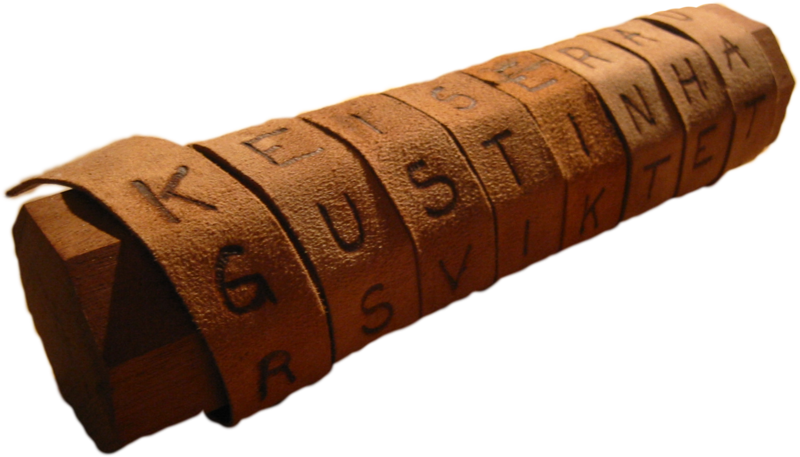
\includegraphics[width=0.5\textwidth]{Immagini/scitala.png}
		\caption{Una ricostruzione di scitala.}
		\label{fig:scitala}
	\end{figure}

\section{Crittosistemi}

	\begin{defn}{Crittosistema}{crittosistema}\index{Crittosistema}
	Un \emph{crittosistema} è una quintupla \((P,C,K,E,D)\), dove
	\begin{itemize}
		\item \(P\) è un insieme finito di testi in chiaro o \emph{plaintext}.
		\item \(C\) è un insieme finito di testi cifrati o \emph{ciphertext}.
		\item \(K\) è un insieme finito di chiavi o \emph{spazio delle chiavi}
		\item Per ogni \(k\in K\) c'è una funzione di cifratura \(e_k\in E\), con \(e_k\colon P \to C\), e una funzione di decifratura \(d_k\in D\), con \(d_k\colon C \to P\), tali che
			\[
			d_k\big(e_k(x)\big) = x
			\]
		per ogni \(x\in P\).
	\end{itemize}
	\end{defn}
	
	\begin{oss}
	Chiaramente se \(x,y\in P\) con \(x\neq y\), si deve avere che, per ogni chiave \(k\),
		\[
		e_k(x) \neq e_k(y).
		\]
	Ovvero le funzioni di \(E\) devono essere iniettve.
	\end{oss}

	\begin{ese}[Cifrario additivo]
	Posti \(P,C,K=\Z_{26}\), fissiamo \(k\in[0,25]\) e definiamo
		\[
		e_k(x) = x+k \pmod{26} \qquad\text{e}\qquad d_k(y) = y-k \pmod{26}.
		\]
	Quando \(k=3\) tale cifrario prende il nome di \emph{cifrario di Cesare}.

	Chiaramente possiamo riportarci all'alfabeto identificando \(\Z_{26}\) con le lettere.
	\end{ese}

	Affinché un crittosistema possa essere considerato efficiente e sicuro, si devono soddisfare due proprietà basilari:
	\begin{itemize}
		\item Dev'essere possibile calcolare ogni \(e_k\) e \(d_k\) in modo computazionalmente efficiente.
		\item \emph{Eve} non deve essere in grado di risalire al testo in chiaro (o peggio, alla chiave) dal testo cifrato.
	\end{itemize}
	Nell'esempio dei cifrari additivi descritto poc'anzi, si hanno solamente 26 possibili chiavi.
	Ciò rende il crittosistema incredibilmente insicuro e attaccabile persino a mano.

	Osserviamo che per definizione, \(P\) e \(C\) sono insiemi finiti e le funzioni di cifratura devono essere iniettive.
	Se in un crittosistema si ha \(P=C\), sappiamo che una funzione \(f\colon P \to C = P\) è iniettiva se e soltanto se è suriettiva.
	Quindi tutte le funzioni di cifratura sono biiettive. In tal caso \(E\) sono le permutazioni di \(P\).
	Se \(P\) ha \(n\) elementi avremo che \(E=S_n\) ha \(n!\) elementi.

	\begin{ese}[Cifrari a sostituzioni]
	Posti \(P=C=\Z_{26}\) e \(K=S_{26}\), per ogni \(\p\in K\) avremo
		\[
		e_\p(x) = \p(x) \qquad\text{e}\qquad d_\p(y) = \p^{-1}(y).
		\]
	In questo caso il numero di chiavi è pari a \(26! \approx 4\cdot 10^{26}\).
	Nonostante questo numero sia molto grande, ciò non basta a garantire la sicurezza di questo crittosistema.
	Questo metodo di cifratura lascia infatti inalterate le regolarità della lingua che permettono una facile decifratura.
	\end{ese}

\section{Crittoanalisi}

	Storicamente con il termine \emph{crittonalisi}, si fa riferimento ai metodi di attacco contro un generico crittosistema.

	\begin{defn}{Principio di Kerckhoffs}{principioKerckhoffs}
	Il principio di Kerckhoffs afferma che la sicurezza di un crittosistema non deve dipendere dal tenere celato il crittoalgoritmo ma solo dal tenere celata la chiave.
	\end{defn}

	In altre parole, il principio di Kerckhoffs afferma che nella costruzione di un crittosistema si deve lavorare affinché il sistema rimanga sicuro anche nell'ipotesi che l'attaccante conosca l'algoritmo di crittazione. Tale principio ha diversi vantaggi:
	\begin{itemize}
		\item \'E più facile tenere segreta la chiave.
		\item Se la sicurezza si basa sulla chiave, e la chiave viene scoperta, basta cambiare chiave.
		\item Si può usare lo stesso crittosistema per far comunicare diverse coppie di persone
		\item Un sistema che viene molto studiato (e attaccato) è più sicuro.
		\item Meglio che le debolezze, se ci sono, vengano scoperte e rese pubbliche.
		\item Se l'algoritmo è pubblico, non c’`e rischio di reverse engineering.
		\item Si possono stabilire standard.
	\end{itemize}
	Oggi il principio di Kerckhoffs viene inteso in maniera più forte: l'algoritmo deve essere pubblico.

	Tornando alla crittoanalisi, elenchiamo alcuni tipi di attacco:
	\begin{description}
		\item[Ciphertext only attack] L'attaccante conosce una stringa \(y\) di testo cifrato. Cerca di risalire al testo in chiaro o alla chiave.
		\item[Known plaintext attack] L'attaccante conosce una stringa \(x\) di testo in chiaro e il corrispondente testo cifrato \(y\). Cerca di risalire alla chiave o di decrittare altri testi cifrati.
		\item[Chosen plaintext attack] L'attaccante ha la possibilità di scegliere un testo in chiaro \(x\) e di ottenere il corrispondente testo cifrato \(y\). Cerca di risalire alla chiave o di decrittare altri testi cifrati.
		\item[Chosen ciphertext attack] L'attaccante ha la possibilità di scegliere un testo cifrato \(y\) e di ottenere il corrispondente testo in chiaro \(x\). Cerca di risalire alla chiave.
	\end{description}
%!TEX root = ../main.tex
%%%%%%%%%%%%%%%%%%%%%%%%%%%%%%%%%%%%%%%%%
%
%LEZIONE 02/03/2017 - PRIMA SETTIMANA (2)
%
%%%%%%%%%%%%%%%%%%%%%%%%%%%%%%%%%%%%%%%%%
\chapter{Crittografia a chiave pubblica}
\section{Introduzione}

	Nella crittografia simmetrica, di cui abbiamo dato una breve introduzione nel capitolo precedente, \emph{Alice} e \emph{Bob} condividono la stessa chiave \(k\).
	La chiave è stata scelta e scambiata fra loro prima dell'inizio della comunicazione.
	Tramite la stessa chiave si ha accesso ad una funzione di cifratura \(e_k\) e ad una di decifratura \(d_k\).
	Generalmente \(d_k\) è facilmente ricavabile da \(e_k\); ciò significa che, tipicamente, se si è in grado di cifrare un messaggio allora lo si sa anche decifrare.

	Come già accennato, prima di cominciare a comunicare è necessario scegliere e scambiarsi la chiave segreta tramite un canale sicuro. Se l'avversario intercetta la chiave, la comunicazione viene compromessa.
	L'idea della crittografia a chiave pubblica, o crittografia \emph{asimmetrica}, è proprio quella di ovviare allo scambio della chiave.

	Si cerca quindi di sviluppare un crittosistema in cui, data la funzione di cifratura \(e_k\), sia computazionalmente difficile determinare \(d_k\).
	Così facendo, \emph{Bob} può rendere pubblica la sua funzione di cifratura \(e_k\); tramite questa, \emph{Alice} può scrivergli senza bisogno di accordi preliminari.
	\emph{Bob} è inoltre l'unico che può decifrare il messaggio.

	Concretamente, è necessario che la funzione di cifratura si una \emph{funzione unidirezionale}.
	In seguito ne daremo una definizione precisa, informalmente una funzione invertibile \(f\colon P \to C\), si dice unidirezionale se:
	\begin{itemize}
		\item Dato \(x\in P\), il calcolo di \(f(x)\) è "facile", cioè è realizzabile con una complessità polinomiale.
		\item Per quasi ogni valore di \(y\in C\), il calcolo di \(f^{-1}(y)\) è "difficile", cioè non è realizzabile con una complessità polinomiale.
	\end{itemize}

	\begin{ese}[Funzione unidirezionale]
	Sia \(n=p\,q\) con \(p,q\) numeri primi sufficientemente grandi e sia \(b\) un intero coprimo con \(\j(n)\)\graffito{\(\j(n)\) è la funzione di Eulero di \(n\)}. Consideriamo la seguente funzione
		\[
		f\colon \Z_n \longrightarrow \Z_n, x \longmapsto x^b \pmod{n}
		\]
	\(f\) è una funzione ritenuta unidirezionale.
	\end{ese}

	Sembra evidente che se la funzione è unidirezionale, anche per \emph{Bob} è impossibile decifrare il messaggio.
	Proprio per questo motivo le funzioni usate nella crittografia a chiave pubblica sono le cosiddette \emph{trapdoor one-way function}, ovvero funzioni unidirezionali che si invertono facilmente quando si conosce un'informazione supplementare.
	Tale informazione sarà tenuta segreta da \emph{Bob}, il quale la utilizzerà per decifrare il messaggio.
	Riepilogando avremo
	\begin{itemize}
		\item Una \emph{chiave pubblica}, resa nota a tutti, che verrà utilizzata per cifrare.
		\item Una \emph{chiave privata}, nota solo a \emph{Bob}, che verrà utilizzata per decifrare.
	\end{itemize}

\section{Cenni di teoria della complessità}

	Ci occuperemo ora di stabilire, in maniera piuttosto grossolana, l'efficienza di un algoritmo.
	In questo corso ci occuperemo di algoritmi che operano sugli interi, pertanto l'input sarà costituito da uno o più interi.

	L'efficienza di un algoritmo viene misurata nel tempo necessario a terminare con successo l'algoritmo stesso.
	Più direttamente, per non rendere la stima dipendente dal sistema usato per misurarla, il tempo dipenderà direttamente dalla lunghezza dell'input.
	Nello specifico, misureremo il tempo di esecuzione in base al numero di \emph{operazioni bit elementari} necessarie a completare l'algoritmo.

	\begin{defn}{Operazioni bit}{operazioniBit}\index{Operazioni bit}
	Con \emph{operazioni bit} intendiamo una fra le seguenti:
	\begin{itemize}
		\item Somma di due cifre binarie.
		\item Moltiplicazione di due cifre binarie.
		\item Divisione di un intero a due cifre binarie per una cifra binaria.
		\item Traslazione a sinistra o a destra di una stringa binaria.
	\end{itemize}
	\end{defn}

	Come già sottolineato, a noi interessa stimare approssimativamente il numero di tali operazioni all'interno di un algoritmo.
	Introduciamo ora la notazione \(\bO\) grande per formalizzare i concetti di complessità computazionale.

	\begin{defn}{Notazione \(\bO\) grande}{notazioneOGrande}\index{O grande}
	Siano \(f,g\colon D \to \R^+, \N\subseteq D\).
	Si dice che \(g\) è \emph{dominata} da \(f\) e si scrive \(g\in \bO(f)\), se esistono \(k,N\in\R\) tali che
		\[
		g(x) \le k\,f(x) ,\,\fa x > N.
		\]
	\end{defn}

	\begin{notz}
	Dalla definizione segue che \(\bO(f)\) è l'insieme delle funzioni dominate da \(f\).
	\end{notz}

	\begin{oss}
	In generale se si ha
		\[
		\lim_{n\to \infty} \frac{f(n)}{g(n)} = l \neq 0,
		\]
	allora \(f\in \bO(g)\) e \(g\in \bO(f)\).
	D'altronde può accadere che quest'ultima condizione sia comunque verificata ma che il limite del rapporto non esista. Ad esempio, se \(f(n) = \big(3+(-1)^n\big)n^3\) e \(g(n)=n^3\), chiaramente si ha \(f\in \bO(g)\) e \(g\in \bO(f)\), ma 
		\[
		\lim_{n\to \infty} \frac{f(n)}{g(n)} = \lim_{n\to \infty} \big(3+(-1)^n\big)
		\]
	non esiste.
	\end{oss}

	\begin{ese}
	Poniamo \(D=\N\) e siano \(f(n) = n^5, g(n) = 5n^5+3n+2\).
	Chiaramente \(f\in \bO(g)\) poiché
		\[
		f(n) \le g(n),\,\fa n.
		\]
	D'altronde avremo anche \(g\in \bO(f)\), infatti
		\[
		g(n) = 5n^5+3n+2 \le 5n^5+3n^5+2n^5 = 10n^5 = 10\,f(n),\,\fa n.
		\]
	\end{ese}

	\begin{ese}
	Sia \(f(n) = n^3\log_2 n\).
	Definitivamente si ha \(\log_2 n \le n\), da cui
		\[
		f\in \bO(n^4).
		\]
	\end{ese}

	\begin{pr}
	Siano \(g_1\in \bO(f_1)\) e \(g_2\in \bO(f_2)\), allora
		\[
		g_1+g_2 \in \bO(f_1+f_2).
		\]
	\end{pr}

	\begin{proof}
	Per definizione
		\[
		g_1 \in \bO(f_1) \implies \,\ex k_1,N_1: g_1(x) \le k_1 f_1(x),\,\fa x > N_1.
		\]
	Analogamente
		\[
		g_2 \in \bO(f_2) \implies \,\ex k_2,N_2: g_2(x) \le k_2 f_2(x),\,\fa x > N_2.
		\]
	Siano \(N=\max\{N_1,N_2\}\) e \(k = \max\{k_1,k_2\}\). Allora se \(x>N\) avremo
		\[
		g_1(x)+g_2(x) \le k_1 f_1(x) + k_2 f_2(x) \le k\,\big(f_1(x)+f_2(x)\big).
		\]
	ovvero \(g_1+g_2\in \bO(f_1+f_2)\).
	\end{proof}

	\begin{pr}
	Siano \(g_1\in \bO(f_1)\) e \(g_2\in \bO(f_2)\), allora
		\[
		g_1 g_2 \in \bO(f_1 f_2).
		\]
	\end{pr}

	\begin{proof}
	Analoga alla precedente.
	\end{proof}

	\begin{pr}
	Siano \(g_1\in \bO(f_1)\) e \(c>0\), allora
		\[
		c\,g_1 \in \bO(f_1).
		\]
	\end{pr}

	\begin{proof}
	Analoga alla precedente.
	\end{proof}

	\begin{defn}{Grandezza di un intero}{grandezzaIntero}\index{Grandezza di un intero}
	Definiamo la \emph{grandezza} di un intero \(n\) come la sua lunghezza in notazione binaria \(L_2(n)\).
	\end{defn}

	\begin{oss}
	Se \(2^{k-1}\le n < 2^k\) avremo
		\[
		k-1 \le \log_2 n < k \implies k = L_2(n) = [\log_2 n] + 1,
		\]
	per cui \(L(n) \in \bO(\log_2 n)\).
	\end{oss}

	\begin{ese}
	Se \(n=24\) la sua grandezza è 5, infatti
		\[
		24 = 11000_2
		\]
	\end{ese}
%%%%%%%%%%%%%%%%%%%%%%%%%%%%%%%%%%%%%%%%%%%
%
%LEZIONE 07/03/2017 - SECONDA SETTIMANA (1)
%
%%%%%%%%%%%%%%%%%%%%%%%%%%%%%%%%%%%%%%%%%%%
	Se l'input dell'algoritmo \(A\) è costituito dagli interi \(n_1,\ldots,n_s\), poniamo
		\[
		n = \max\{\abs{n_1},\ldots,\abs{n_s}\} \qquad\text{e}\qquad k=L(n).
		\]
	Con \(T(A)\) definiamo il tempo di esecuzione di \(A\), pari a circa il numero di operazioni bit elementari che servono per l'esecuzione dell'algoritmo.
	\(T(A)\) sarà pertanto una funzione di \(k\). In particolare noi saremo interessati ad una stima del tipo \(T(A)\in \bO\big(f(k)\big)\).

	\begin{defn}{Algoritmo polinomiale}{algoritmoPolinomiale}\index{Algoritmo polinomiale}
	Un algoritmo \(A\) si dice \emph{polinomiale} se esiste \(d\ge 1\) tale che
		\[
		T(A) \in \bO(k^d).
		\]
	\end{defn}

	\begin{notz}
	L'esponente \(d\) si dice \emph{ordine di \(A\)}.
	\end{notz}

	\begin{defn}{Algoritmo esponenziale}{algoritmoEsponenziale}\index{Algoritmo esponenziale}
	Un algoritmo \(A\) si dice \emph{esponenziale} se esiste \(c>0\) tale che
		\[
		T(A) \in \bO(2^{c\,k}).
		\]
	\end{defn}

	\begin{notz}
	Diremo che \(A\) è \emph{sottoesponenziale} se
		\[
		T(A) \in \bO(2^{f(k)}) \qquad\text{dove } \lim_{n \to \infty} \frac{f(n)}{n} = 0.
		\]
	\end{notz}
\section{Calcolo della complessità di algoritmi noti}

	In questo paragrafo studieremo la complessità computazionale di alcuni algoritmi basilari e/o noti.

	In generale faremo riferimento ad \(a\) e \(b\) come due interi con \(a \ge b\), inoltre denoteremo
		\[
		L(a) = k \qquad\text{e}\qquad L(b) = h.
		\]

	\begin{prop}{Complessità della somma}{complessitàSomma}
	Consideriamo l'algoritmo per la somma di due interi \(a+b\), allora
		\[
		T(a+b) \in \bO(k).
		\]
	\end{prop}

	\begin{proof}
	Una somma fra due interi è compiuta attraverso \(k\) somme elementari tra i bit che li compongono.
	Eventualmente tali somme potrebbero causare un riporto che necessita di un'ulteriore somma.
	Al più vi saranno quindi \(2k\) operazioni bit. Ne segue
		\[
		T(a+b) \in \bO(k).\qedhere
		\]
	\end{proof}

	\begin{oss}
	Analogamente si mostra \(T(a-b)\).
	\end{oss}

	\begin{prop}{Complessità della moltiplicazione}{complessitàMoltiplicazione}
	Consideriamo l'algoritmo per il prodotto di due interi \(a\,b\), allora
		\[
		T(a\,b) \in \bO(k^2).
		\]
	\end{prop}

	\begin{proof}
	Per ognuna delle \(h\) cifre di \(b\) bisogna eseguire \(k\) moltiplicazioni elementari tra bit, per un totale di \(h\,k\) moltiplicazioni elementari.
	Infine è necessario compiere \(h-1\) somme tra i prodotti parziali precedentemente calcolati.
	Per la proposizione precedente sappiamo che la somma ha una complessità lineare ed ha pertanto un ordine inferiore rispetto alle moltiplicazioni precedenti. Quindi
		\[
		T(a\,b) \in \bO(h\,k) \subseteq \bO(k^2).\qedhere
		\]
	\end{proof}

	\begin{oss}
	Esistono altri algoritmi che eseguono il prodotto fra interi in modo più efficiente, raggiungendo una complessità che è circa \(\bO(k^{1,5})\).
	\end{oss}

	\begin{prop}{Complessità della divisione}{complessitàDivisione}
	Consideriamo l'algoritmo della divisione con resto fra interi \(a/b\), allora
		\[
		T(a/b) \in \bO(k^2).
		\]
	\end{prop}

	\begin{proof}
	L'algoritmo della divisione con resto è quello "classico" della divisione in colonna.
	Ad ogni passaggio si confronta il dividendo con il resto della divisione precedente; questo confronto, nel caso binario, può dare \(1\) se il divisore coincide con il dividendo o \(0\) altrimenti. Dopodiché si fanno \(h\) moltiplicazioni del risultato del confronto per le \(h\) cifre di \(b\) e si sottrae il risultato al resto precedente.

	Complessivamente si fanno \(h\) moltiplicazioni per la lunghezza del quoziente e altrettante sottrazioni. Le sottrazioni sono di un ordine più basso rispetto alle moltiplicazioni, resta quindi da stimare la lunghezza del quoziente.
		\[
		a = b\,q +r \implies L(a) = L(b\,q) + L(r).
		\]
	Osserviamo che, in generale, se \(a\ge b\), avremo
		\[
		L(a+b)  = 	\begin{cases}
					L(a)\\
					L(a)+1
					\end{cases}
		\qquad\text{e}\qquad
		L(a\,b) = 	\begin{cases}
					L(a)+L(b)-1\\
					L(a)+L(b)
					\end{cases}
		\]
	Considerando i casi computazionalmente peggiori e ricordando che \(r<b\), avremo
		\[
		L(a) = L(b\,q)+L(r) = L(b\,q)+1 = L(b)+L(q)+1 \implies L(q) = L(a)-L(b) < L(a).
		\]
	Per cui abbiamo \(h\,k\) operazioni elementari, da cui
		\[
		T(a/b) \in \bO(k^2).\qedhere
		\]
	\end{proof}

	\begin{prop}{Complessità dell'algoritmo euclideo}{complessitàAlgoritmoEuclideo}
	Consideriamo l'algoritmo euclideo per il calcolo del MCD, allora
		\[
		T\big((a,b)\big) \in \bO(k^3).
		\]
	\end{prop}

	\begin{proof}
	In generale possiamo supporre \(a>b>0\).
	Chiamiamo \(r_0=a\) e \(r_1=b\). Tramite la divisione col resto otteniamo
		\begin{gather*}
		r_0 = q_1 r_1 + r_2,\\
		r_1 = q_2 r_2 + r_3,\\
		...
		\end{gather*}
	Iterando questo procedimento, al passo \(i\) avremo
		\[
		r_{i-1} = q_i r_i + r_{i+1}.
		\]
	Dopo un certo numero di passi, che siamo sicuri essere finito poiché \(r_1 > r_2 > \ldots\), arriveremo a
		\[
		r_{m-1} = q_m r_m + 0 \implies (a,b) = r_m.
		\]
	Quindi nell'algoritmo vengono compiute \(m\) divisioni.
	Poiché di queste ultime conosciamo già il peso computazionale, dobbiamo stimare \(m\) in termini di \(k\).

	Lo scenario computazionalmente peggiore è quello in cui il resto diminuisca sempre di \(1\).
	In questo caso \(m\) sarebbe confrontabile con \(b \approx 2^h\). Se questa fosse la migliore stima, la complessità di \((a,b)\) sarebbe esponenziale.
	
	Cerchiamo quindi una stima migliore per \(m\). Consideriamo i primi tre passi:
		\[
		a = b\,q + r, \qquad b = q'r + r' \qquad r = q'' r' + r'',
		\]
	e mostriamo che \(2r \le a\). Ci sono due casi:
	\begin{itemize}
		\item Se \(q=1\) avremo \(r= a-b\). Inoltre \(q=1\) può avvenire solo se \(b > a/2\), da cui
			\[
			r < \frac{a}{2}.
			\]
		\item Se \(q > 1\) necessariamente \(b \le a/2\), da cui
			\[
			r < b \le \frac{a}{2}.
			\]
	\end{itemize}
	Pertanto \(2r \le a\). In generale
		\[
		2 r_{i+2} \le r_i \implies m \le \lfloor \log_2 a \rfloor +1,
		\]
	che ci permette di concludere
		\[
		T\big((a,b)\big) \in \bO(k^3).\qedhere
		\]
	\end{proof}
%%%%%%%%%%%%%%%%%%%%%%%%%%%%%%%%%%%%%%%%%%%
%
%LEZIONE 08/03/2017 - SECONDA SETTIMANA (2)
%
%%%%%%%%%%%%%%%%%%%%%%%%%%%%%%%%%%%%%%%%%%%
\section{Problemi P e NP}

	Introduciamo brevemente la classe di problemi \(P\) e \(NP\) per poi valutarne l'applicabilità ad eventuali algoritmi crittografici.

	\begin{defn}{Problemi \(P\)}{problemiP}
	Definiamo \(P\) la classe di problemi per cui esiste un algoritmo che risolve il dato problema in tempo \emph{polinomiale}.
	\end{defn}

	\begin{defn}{Problemi \(NP\)}{problemiNP}
	Definiamo \(NP\) la classe di problemi per cui esiste un algoritmo che li risolve (non necessariamente in tempo polinomiale) e tali che, un'eventuale soluzione può essere verificata in tempo polinomiale.
	\end{defn}

	\begin{oss}
	Chiaramente si ha \(P\subseteq NP\). Uno dei problemi centrali della teoria della complessità è proprio stabilire se
		\[
		P \neq NP.
		\]
	\end{oss}

	\begin{defn}{Problemi \(NP\)-completi}{}
	Un problema \(\p\) di classe \(NP\) si dice \(NP\)-completo se, per ogni problema \(\p'\in NP\), esiste un algoritmo che riduce la soluzione di \(\p'\) ad una di \(\p\) in tempo polinomiale.
	\end{defn}

	\begin{oss}
	Se esistesse un algoritmo che risolve un problema \(NP\)-completo in tempo polinomiale, si avrebbe immediatamente
		\[
		P = NP.
		\]
	I problemi \(NP\)-completi sono quindi, di fatto, i problemi computazionalmente più difficili tra quelli di classe \(NP\).
	\end{oss}
\section{Problema dello zaino}

	In questo paragrafo studieremo un problema \(NP\)-completo e una sua applicazione nella crittografia a chiave pubblica.

	Supponiamo di avere uno zaino che possa contenere \(b\) unità e una lista di oggetti di volume \(a_1, \ldots, a_k\).
	Il problema dello zaino è riempire completamente lo zaino, formalmente dobbiamo trovare una \(k\)-pla
		\[
		e = (e_1, \ldots, e_k) \qquad\text{con }e_i \in \{0,1\},
		\]
	tale che
		\[
		b = \sum_{i=1}^k e_i a_i;
		\]
	oppure mostrare che tale \(k\)-pla non esiste.

	\'E facile osservare che si tratta di un problema computazionalmente difficile, dati \(k\) oggetti vi sono infatti \(2^k\) possibili combinazioni di tali oggetti.
	Nonostante ci siano algoritmi più efficienti, non ne esiste nessuno polinomiale.
	D'altronde la verifica di una possibile soluzione avviene in tempo lineare, pertanto il problema dello zaino è un problema di classe \(NP\). Si dimostra inoltre essere \(NP\)-completo.

	Affinché vi sia una rilevanza dal punto di vista crittografico, dobbiamo identificare dei casi in cui la risoluzione del problema dello zaino sia computazionalmente facile. Definiamo quindi un particolare tipo di successioni per cui ciò avviene

	\begin{defn}{Successioni supercrescenti}{successioniSupercrescenti}
	Una successione \((a_1,\ldots,a_k)\) si dice \emph{supercrescente} se ogni termine è maggiore della somma dei precedenti, ovvero se
		\[
		a_i > \sum_{j=1}^{i-1} a_j.
		\]
	\end{defn}
	\noindent
	Il motivo per cui una successione supercrescente rende facile il problema dello zaino è che, per verificare se una soluzione esiste, è sufficiente inserire nello zaino gli oggetti più grandi possibili.
	Infatti se l'oggetto \(a_i\) fosse il più grande inseribile nello zaino, anche se scegliessimo di inserire tutti gli oggetti che lo precedono al suo posto, otterremo comunque una grandezza più piccola di \(a_i\).
	Questo ci garantisce inoltre che la soluzione, se esiste, è unica.

	\begin{ese}
	Consideriamo la seguente successione supercrescente
		\[
		(1,2,4,8,16,32).
		\]
	Cerchiamo di riempire uno zaino con \(b=45\) utilizzando la strategia enunciata prima, anche detta "greedy":
	\[
	45 = 32+\emph{13} = 32+8+\emph{5} = 32+8+4+1.
	\]
	\end{ese}
\section{Crittosistema di Merkle-Hellman}

	Il crittosistema di Merkle-Hellman si basa sul problema dello zaino e sfrutta un mascheramento delle successioni supercrescenti per costruire la chiave privata.

	L'idea di base è la seguente:
	\begin{itemize}
		\item La chiave privata è costituita da una successione \((a_1,\ldots,a_k)\).
		\item Il messaggio, per essere cifrato, deve essere una stringa binaria \((e_1,\ldots,e_k)\) di \(k\) elementi.
		\item Il messaggio cifrato è
			\[
			b = \sum_{i=1}^k e_i a_i
			\]
		dove sappiamo che \(e_i\in\{0,1\}\).
	\end{itemize}
	In questo modo, per decifrare il messaggio bisognerebbe risolvere un problema dello zaino.
	D'altronde in queste condizioni il messaggio non può essere decifrato neppure da Bob.

	Dobbiamo quindi sfruttare le proprietà sulle successioni supercrescenti che abbiamo visto nel precedente paragrafo.
	Chiaramente la chiave pubblica non può essere una successione supercrescente, altrimenti chiunque potrebbe decifrare il messaggio. \'E necessario mascherare questa proprietà.

	Bob sceglie una successione supercrescente \((a_1,\ldots,a_k)\). Sceglie inoltre due interi \(n\) e \(u<n\) tali che
		\[
		n > \sum_{i=1}^k a_i \qquad\text{e}\qquad (u,n) = 1.
		\]
	Attraverso questi ultimi costruisce una nuova successione \((a_1^*,\ldots,a_k^*)\) tale che
		\[
		a_i^* \equiv u\,a_i \pmod{n}.
		\]
	Così facendo avremo
	\begin{itemize}
		\item \((a_1,\ldots,a_k), n\) e \(u\) la chiave privata.
		\item \((a_1^*, \ldots a_k^*)\) la chiave pubblica.
	\end{itemize}
	La cifratura avviene come descritto prima, Alice invia 
		\[
		b^* = \sum_{i=1}^k e_i a_i^*.
		\]
	Per decifrare, Bob calcola \(v\), l'inverso moltiplicativo di \(u\) modulo \(n\).
	Tramite \(v\) calcola
		\[
		b = v\,b^* \pmod{n}.
		\]
	Ora
		\[
		\begin{split}
		b & \equiv v\,b^* \equiv v\, \sum_{i=1}^k e_i a_i^* \equiv v \,\sum_{i=1}^k e_i u\,a_i\equiv v\,u\,\sum_{i=1}^k e_i a_i\\
		& \equiv \sum_{i=1}^k e_i a_i \pmod{n}
		\end{split}
		\]
	Inoltre sia \(b\) che \(\sum_{i}e_i a_i\) sono minori di \(n\), per cui
		\[
		b \equiv_n \sum_{i=1}^k e_i a_i \implies b = \sum_{i=1}^k e_i a_i.
		\]
	A questo punto Bob deve risolvere un problema dello zaino facile per decifrare il messaggio.

	\begin{ese}
	Come chiave privata utilizziamo
		\[
		(1, 3, 7, 15, 31, 63, 127, 255), \qquad n=557, \qquad u=323.
		\]
	Osserviamo che, come da condizione, \(n\) è maggiore della somma della successione e \(u\) è coprimo con \(n\).
	Moltiplicando ogni termine della successione supercresente per \(u\) e riducendo modulo \(n\), si ottiene la chiave pubblica
		\[
		(323, 412, 33, 389, 544, 297, 360, 486).
		\]
	Supponiamo di voler cifrare la stringa binaria \(01100101\) che ha lunghezza \(8\) come la chiave. Otterremo la codifica
		\[
		b^* = 0\cdot323+1\cdot412+1\cdot33 + 0\cdot389 + 0\cdot544 + 1\cdot297 + 0\cdot360 + 1\cdot486 = 1228.
		\]
	Bob riceve \(b^*\). Calcola \(v=169\) l'inverso di \(u\) modulo \(n\) per ottenere
		\[
		 b = v\,b^* \equiv 328 \pmod{n}.
		\]
	Risolve il problema dello zaino con \(b=328\) e la sua successione supercrescente:
		\[
		328 = 255 + \emph{73} = 255+63 + \emph{10} = 255+63+7+3.
		\]
	Confrontando con i termini presenti nella successione supercrescente riottiene la stringa \(01100101\).
	\end{ese}

	Il crittosistema che abbiamo descritto in questo paragrafo è stato sviluppato da Merkle e Hellman nel 1978.
	\'E un sistema molto elegante, molto più semplice di sistemi come l'RSA.
	D'altronde venne violato piuttosto in fretta, nel 1984 Shamir pubblicò un articolo in cui esponeva un algoritmo che forzava il crittosistema in tempo polinomiale.
%!TEX root = ../main.tex
%%%%%%%%%%%%%%%%%%%%%%%%%%%%%%%%%%%%%%%%%%%
%
%LEZIONE 08/03/2017 - SECONDA SETTIMANA (3)
%
%%%%%%%%%%%%%%%%%%%%%%%%%%%%%%%%%%%%%%%%%%%
\chapter{Il crittosistema RSA}
	
	In questo capitolo descriveremo in dettaglio il crittosistema RSA.
	Nella parte iniziale richiameremo e svilupperemo alcuni concetti matematici e computazionale che ci saranno utili in seguito.

\section{Introduzione}

	In questo paragrafo richiameremo alcuni fatti di teoria modulare e analizzeremo l'algoritmo di esponenziazione modulare.

	\begin{teor}{di Eulero-Fermat}{teoremaEuleroFermat}
	Siano \(a\in \Z\) e \(n\in\N\) tali che \((a,n)=1\). Allora
		\[
		a^{\j(n)} \equiv 1 \pmod{n}.
		\]
	\end{teor}

	\begin{oss}
	Un caso particolare si ha quando \(n=p\) primo. In tal caso se \(p\nmid a\) si ha \((a,p)=1\) e in particolare
		\[
		a^{\j(p)} = a^{p-1} \equiv 1 \pmod{p} \iff a^p \equiv a \pmod{p}.
		\]
	\end{oss}

	\begin{notz}
	\(\j(n)\) è la funzione di Eulero calcolata in \(n\), ovvero il numero di interi minori di \(n\) e coprimi con esso. Ricordiamo che in generale se \(n=p_1^{\a_1} \cdot\ldots\cdot p_s^{\a_s}\) avremo
		\[
		\j(n) = \j(p_1^{\a_1}) \cdot\ldots\cdot \j(p_s^{\a_s}) = p_1^{\a_1-1}(p_1-1) \cdot\ldots\cdot p_s^{\a_s-1}(p_s-1).
		\]
	Per cui è possibile calcolare \(\j(n)\) se si conosce la fattorizzazione di \(n\).
	\end{notz}

	\begin{cor}\label{cor:teoremaFermatRSA}
	Sia \(n=p\,q\) con \(p,q\) primi. Sia \(m\equiv 1 \pmod{\j(n)}\). Allora
		\[
		a^m \equiv a \pmod{n},\,\fa a \in \Z.
		\]
	\end{cor}

	\begin{proof}
	La tesi è banalmente vera per Eulero se \((a,n)=1\). Supponiamo quindi che \((a,n)>1\).
	Passando in modulo \(p\), vi sono due possibilità:
	\begin{itemize}
		\item Se \(p\mid a\) allora
			\[
			a^m \equiv a \equiv 0 \pmod{p}.
			\]
		\item Se \(p\nmid a\), per ipotesi abbiamo \(m\equiv 1 \pmod{\j(n)}\) dove \(\j(n)=(p-1)(q-1)\), quindi
			\[
			a^m = a^{1+k(p-1)(q-1)} = a\,(a^{p-1})^{k\,(q-1)} \equiv a \pmod{p}.
			\]
	\end{itemize}
	Analogamente si mostra \(a^m \equiv a \pmod{q}\), da cui
		\[
		\begin{cases}
		a^m \equiv a \pmod{p}\\
		a^m \equiv a \pmod{q}
		\end{cases}
		\implies a^m \equiv a \pmod{n},
		\]
	per il teorema cinese dei resti.
	\end{proof}

	In generale, se vogliamo calcolare \(a^n\), dobbiamo eseguire \(n-1\) moltiplicazioni.
	Se \(n\approx 2^k\) questo significa che la complessità dell'esponenziazione è esponenziale.
	Per ridurre tale complessità, l'idea è scrivere \(n\) come somma di potenze di 2 e spezzare la potenza.
	Supponiamo di avere
		\[
		n = 2^k + 2^{k-i} + \ldots + 2^{k-m} \implies a^k = a^{2^k}a^{2^{k-i}} \cdot\ldots\cdot a^{2^{k-m}}.
		\]
	A questo punto è sufficiente calcolare le potenze di \(a\) fino a \(a^{2^k}\), nel processo calcoleremo incidentalmente anche tutte quelle precedenti. Infine basta moltiplicare fra di loro le potenze trovate.
	Osserviamo in particolare che per calcolare ogni potenza è sufficiente una singola moltiplicazione, infatti
		\begin{align*}
		a^2 & = a \cdot a;\\
		a^{2^2} & = a^2 \cdot a^2;\\
		& \ldots\\
		a^{2^k} & = a^{2^{k-1}} \cdot a^{2^{k-1}}.
		\end{align*}

	A noi interessa valutare la complessità di questo algoritmo nel caso modulare

	\begin{prop}{Complessità dell'algoritmo square and multiply}{complessitàSquareMultiply}
	Siano \(b,m,n\in \Z\) con \(L(m) = k\) e \(L(n) = h\).
	Consideriamo l'algoritmo \(A\) per il calcolo di \(b^m \pmod{n}\) tramite la strategia precedente, allora
		\[
		T(A) \in \bO\big((k-1)h^2\big).
		\]
	\end{prop}

	\begin{proof}
	Supponiamo di avere
		\[
		m = a_0 + a_1 2 + a_2 2^2 + \ldots + a_{k-1}2^{k-1} \qquad\text{con }a_i \in \{0,1\}.
		\]
	Pertanto avremo
		\[
		b^m = b^{a_0+a_1 2 + \ldots + a_{k-1}2^{k-1}} = b^{a_0}b^{a_1 2} \cdot\ldots\cdot b^{a_{k-1}2^{k-1}}.
		\]
	Dobbiamo calcolare le \(k\) potenze di \(2\). Come osservato in precedenza il calcolo di \(2^i\) è costituito da una singola moltiplicazione di numeri minori di \(n\). Nel caso computazionalmente peggiore, ovvero se \(a_i=1\) per ogni \(i\), avremo \(k-1\) passi.
	Quindi, ricordando la complessità della moltiplicazione, avremo
		\[
		T(A) \in \bO\big((k-1)h^2\big).
		\]
	\end{proof}

	\begin{oss}
	Se si ha \((b,n)=1\), possiamo supporre che \(m \le \j(n)\). Infatti se così non fosse, potrei scrivere
		\[
		b^m \equiv b^{m'} \pmod{n} \qquad\text{con } m \equiv m' \pmod{\j(n)}.
		\]
	Pertanto se \((b,n)=1\) avremo \(m \le \j(n) \le n\), ovvero \(L(m) \le L(n)\).
	Quindi la complessità dell'esponenziazione può essere stimata completamente in termini di \(h=L(n)\), ottenendo
		\[
		T(A) \in \bO(h^3).
		\]
	\end{oss}
%%%%%%%%%%%%%%%%%%%%%%%%%%%%%%%%%%%%%%%%%
%
%LEZIONE 14/03/2017 - TERZA SETTIMANA (1)
%
%%%%%%%%%%%%%%%%%%%%%%%%%%%%%%%%%%%%%%%%%
\section{Descrizione del crittosistema}

	Come ogni crittosistema a chiave pubblica, anche RSA si basa su una funzione unidirezionale speciale.
	L'idea del crittosistema si basa sulla difficoltà nella fattorizzazione dei numeri.
	In particolare abbiamo visto come moltiplicare due interi a \(n\) bit sia dell'ordine di \(\bO(n^2)\), mentre è possibile dimostrare che fattorizzare un numero a \(n\) bit è un'operazione dell'ordine di \(\bO(2^{c\,n^{1/3}})\).

	Il crittosistema RSA si schematizza come segue:
	\begin{itemize}
		\item Sia \(N=p\,q\) con \(p,q\) primi e siano \(P=C=\Z_N\).
		\item Lo spazio delle chiavi è
			\[
			K = \Set{(N,p,q,d,e) | d\,e \equiv 1 \pmod{\j(N)}}.
			\]
	\end{itemize}

	Da questo insieme avremo
	\begin{itemize}
		\item \((p,q,d)\) la chiave privata.
		\item \((N,e)\) la chiave pubblica.
	\end{itemize}

	Se \(k=(N,p,q,d,e)\) è una chiave, il messaggio \(x\in P\) verrà criptato attraverso
		\[
		e_k(x) = x^e \pmod{N}.
		\]
	Viceversa, un codice \(y\in C\) sarà decriptato con
		\[
		d_k(y) = y^d \pmod{N}.
		\]
	Dalla costruzione della chiave, sappiamo che \(e\,d \equiv 1 \pmod{\j(N)}\), inoltre \(N=p\,q\) con \(p,q\) primi.
	Quindi per il \hyperref[cor:teoremaFermatRSA]{corollario di Fermat} sappiamo che
		\[
		(x^e)^d \equiv x \pmod{N} \iff d_k(e_k(x)) = x.
		\]

	\begin{ese}
	Supponiamo che Bob scelga \(p=17\) e \(q=11\), costruisce quindi
		\[
		N = 17\cdot 11 = 187 \qquad\text{e}\qquad \j(N) = 16\cdot 10 = 160.
		\]
	Bob scegli inoltre \(e=7\) e calcola \(d=e^{-1}=23 \pmod{160}\).
	Pubblica quindi la chiave pubblica \((187,7)\).

	Supponiamo che Alice voglia cifrare il testo in chiaro \(88\), il cifrato sarà quindi
		\[
		88^7 = 11 \pmod{187}.
		\]
	Bob riceve \(11\) da Alice, per decifrare calcola
		\[
		11^{23} = 88 \pmod{187}
		\]
	ritrovando quindi il messaggio originale.
	\end{ese}
	\noindent
	Alla base dell'RSA vi sono quindi una serie di problemi "facili" in fase di cifratura e "difficili" in decifratura.
	Nei prossimi paragrafi ci occuperemo proprio di studiare algoritmi polinomiali per i problemi di cifratura e di dimostrare che tutti i problemi di decifratura sono equivalenti alla fattorizzazione di un intero.

	In particolare i problemi che coinvolgono la cifratura sono
	\begin{itemize}
		\item Determinare se un intero \(n\) è primo.
		\item Dati \(a\) e \(n\), trovare \((e,n)\) e, nel caso \((e,n)=1\), calcolare l'inverso di \(e\) modulo \(n\).
		\item Calcolare la funzione \(x^e \pmod{n}\).
	\end{itemize}
	Degli ultimi due problemi abbiamo già esibito un algoritmo polinomiale, rispettivamente l'algoritmo di Euclide e l'algoritmo square and multiply.
	Ai cosiddetti test di primalità, dedicheremo il prossimo paragrafo.

	Viceversa, i problemi che coinvolgono la decifratura sono
	\begin{itemize}
		\item Fattorizzare un intero \(n\).
		\item Dato un intero \(n\), calcolare \(\j(n)\).
		\item Dati \(n,e\), trovare \(d\) tale che
			\[
			(x^e)^d \equiv x \pmod{n}.
			\]
	\end{itemize}

	A prima vista questi problemi sono esposti in ordine di difficoltà. \'E chiaro infatti che se si riesce a fattorizzare \(n\), gli altri due problemi diventano banali.
	Questo ci fa capire che violare l'RSA non può essere più difficile che fattorizzare un intero.
	D'altronde, vedremo in seguito che questi tre problemi sono tra loro equivalenti.

\section{Test di primalità}

	In questo paragrafo ci occuperemo di descrivere alcuni algoritmi polinomiali per determinare se un interno \(n\) sia primo.
	Come è facile intuire, affinché questi algoritmi siano polinomiali, essi non forniranno alcuna informazione sulla fattorizzazione di \(n\).

	Nella prima parte faremo cenno ad alcuni elementi di teoria dei numeri, per una trattazione più approfondita si consiglia di fare riferimento ad un testo specializzato.

	\begin{teor}{Cardinalità numeri primi}{cardinalitàNumeriPrimi}
	Vi sono infiniti numeri primi.
	\end{teor}

	\begin{proof}
	Supponiamo per assurdo che vi siano un numero finito di primi \(p_1,\ldots,p_k\).
	Definiamo
		\[
		N = p_1 \cdot\ldots\cdot p_k +1.
		\]
	Per costruzione \(N\) non è divisibile per nessuno dei \(p_1,\ldots,p_k\).
	Per cui vi sono altri primi che fattorizzano \(N\), da cui l'assurdo.
	\end{proof}

	\begin{teor}{dei numeri primi}{teoremaNumeriPrimi}
	Sia \(\p(x)\) la funzione aritmetica che enumera i numeri primi fino ad \(x\). Allora
		\[
		\lim_{x \to \infty} \frac{\p(x)}{\frac{x}{\ln x}} = 1
		\]
	\end{teor}

	\begin{oss}
	Tramite il teorema dei numeri primi, è possibile stimare la probabilità che un numero \(N\) sia primo. Tale probabilità è infatti circa
		\[
		\p(N)/N.
		\]
	Ad esempio, la probabilità che un numero casuale con al più cento cifre decimali sia primo è circa
		\[
		\frac{1}{\ln(10^{100})} = \frac{1}{230}.
		\]
	Questa probabilità può essere raffinata, scartando ad esempio i numeri pari e i multipli di tre, scarteremmo \(\frac{2}{3} = \frac{1}{2}+\frac{1}{6}\). La probabilità di trovare un primo con al più cento cifre diventa quindi \(\frac{1}{77}\).

	Questo ci dice che trovare numeri primi di grandi dimensioni è relativamente facile.
	\end{oss}

	\begin{defn}{Numero di Fermat}{numeroFermat}\index{Numero!di Fermat}
	Un numero si dice \emph{di Fermat} se è della forma
		\[
		F_n = 2^{2^n}+1.
		\]
	\end{defn}

	\begin{ese}
	\(F_0=3,F_1=5,F_2=17\) sono numeri di Fermat.
	\end{ese}

	\begin{oss}
	Fermat congetturò che \(F_n\) è primo per ogni \(n\).
	Ciò venne velocemente dimostrato falso fattorizzando \(F_5\).
	\end{oss}

	\begin{prop}{Espressione ricorsiva dei numeri di Fermat}{espressioneRicorsivaNumeriFermat}
	Siano \(F_i\) i numeri di Fermat, allora
		\[
		F_n-2 = \prod_{i=0}^{n-1} F_i.
		\]
	\end{prop}

	\begin{proof}
	Mostriamolo per induzione:
	\begin{itemize}
		\item Per \(n=1\) è banalmente vero, infatti
			\[
			F_1 -2 = 5-2 = 3 = F_0.
			\]
		\item Supponiamo che la tesi sia vera per \(n-1\) e mostriamola per \(n\):
			\[
			\begin{split}
			F_n-2 & = 2^{2^n}+1-2 = 2^{2^n}-1 = \big(2^{2^{n-1}}\big)^2-1 = \big(2^{2^{n-1}}-1\big)\big(2^{2^{n-1}}+1\big)\\
			& = \big(2^{2^{n-1}}+1-2\big)\big(2^{2^{n-1}}+1\big) = (F_{n-1}-2)\,F_{n-1}.
			\end{split}
			\]
		Ma per ipotesi induttiva
			\[
			F_{n-1}-2 = \prod_{i=0}^{n-2}F_i,
			\]
		da cui
			\[
			F_n -2 = \left( \prod_{i=0}^{n-2}F_i \right)\,F_{n-1} = \prod_{i=0}^{n-1}F_i.\qedhere
			\]
	\end{itemize}
	\end{proof}

	\begin{cor}
	Siano \(F_n,F_m\) due numeri di Fermat con \(n\neq m\). Allora
		\[
		(F_n,F_m) = 1.
		\]
	\end{cor}

	\begin{proof}
	Supponiamo per assurdo che \(p\) sia un primo che divide sia \(F_n\) che \(F_m\), dove assumiamo \(n<m\) senza perdita di generalità.
	Dal momento che \(p\mid F_n\) avremo
		\[
		p \mid F_0 \cdot\ldots\cdot F_n \cdot\ldots\cdot F_{m-1}.
		\]
	Inoltre, dalla proposizione precedente,
		\[
		p \mid F_m = F_0 \cdot\ldots\cdot F_{m-1} +2.
		\]
	Quindi \(p\) deve dividere la differenza fra \(F_0 \cdot\ldots\cdot F_{m-1}+2\) e \(F_0 \cdot\ldots\cdot F_{m-1}\) che è \(2\).
	Da cui \(p=2\) che è assurdo in quanto i numeri di Fermat sono per costruzione dispari.
.	\end{proof}

	\begin{oss}
	Da questo corollario segue una dimostrazione alternativa sull'infinità dei numeri primi: infatti, dal momento che esistono infiniti numeri di Fermat e che ogni numero primo ne divide al più uno solo, devono esistere infiniti numeri primi.
	\end{oss}

	\begin{defn}{Test deterministico}{testDeterministico}\index{Test!deterministico}
	Un test si dice \emph{deterministico} se risponde in modo univoco ad un problema, senza margine di errore.
	\end{defn}

	\begin{defn}{Test probabilistico}{testProbabilistico}\index{Test!probabilistico}
	Un test si dice \emph{probabilistico} se consiste di una successione di test \(\{T_m\}_{m\in\N}\) e una successione che tende a zero \(\{\e_m\}_{m\in\N}\) tale che:
	\begin{itemize}
		\item Se il problema non passa un test \(T_m\) allora la risposta è certamente negativa.
		\item La probabilità che il problema superi di test \(T_1, \ldots, T_m\) ma che la risposta sia negativa è minore di \(\e_m\).
	\end{itemize}
	\end{defn}

	\begin{oss}
	Fino al 2002 gli unici test di primalità polinomiali erano probabilistici.
	Nel 2002, venne trovato un algoritmo polinomiale per determinare la primalità con una complessità computazionale di \(\bO(n^{12})\) in seguito migliorata a \(\bO(n^6)\).
	Da ciò sappiamo che il problema di primalità è un problema \(P\).
	\end{oss}

	Dal punto di vista dell'efficienza si preferisce usare un test di primalità probabilistico, in quanto più veloce e sufficientemente affidabile.
	L'idea di un test di primalità probabilistico è quello di cercare prove del fatto che \(n\) si comporti o meno come un primo senza cercare i suoi fattori.
	Si utilizzano quindi condizioni necessarie dei numeri primi, che in caso di fallimento ci garantiscono la non primalità di \(n\), mentre in caso di successo aumentano la probabilità che \(n\) sia primo.

\subsection{Test di Fermat}

	Il test di Fermat è un test di primalità probabilistico che sfrutta il \hyperref[th:teoremaEuleroFermat]{teorema di Fermat}. Ricordiamo che quest'ultimo afferma che, se \(p\) è primo e \(1\le a <p\), allora
		\[
		a^{p-1} \equiv  1 \pmod{p}.
		\]
	Sia \(n\) è l'intero di cui vogliamo determinare la primalità, se troviamo \(a < n\) tale che
		\[
		a^{n-1} \not\equiv 1 \pmod{n},
		\]
	allora sappiamo per certo che \(n\) non è primo pur non avendo studiato i suoi fattori.

	Il test di Fermat per \(n\in\N\) è quindi il seguente:
	prendiamo \(a<n\) e calcoliamo \((a,n)\),
	\begin{itemize}
		\item Se \((a,n)\neq 1\) allora \(n\) non è primo;
		\item Se \((a,n)=1\) calcoliamo \(a^{n-1}\) modulo \(n\). Se è diverso da \(1\) allora \(n\) non è primo. 
	\end{itemize}

	\begin{ese}
	Valutiamo la primalità di \(323\):
		\[
		2^{322} \equiv 157 \pmod{323},
		\]
	quindi \(323\) non è primo.
	\end{ese}
%%%%%%%%%%%%%%%%%%%%%%%%%%%%%%%%%%%%%%%%%
%
%LEZIONE 16/03/2017 - TERZA SETTIMANA (2)
%
%%%%%%%%%%%%%%%%%%%%%%%%%%%%%%%%%%%%%%%%%
	\begin{defn}{Pseudoprimo}{pseudoprimo}\index{Pseudoprimo}
	Si dice che \(n\) è uno \emph{pseudoprimo in base \(a\)}, se \(n\) non è primo ma
		\[
		a^n \equiv a \pmod{n}.
		\]
	\end{defn}

	\begin{oss}
	Il nome pseudoprimo si usa in quanto il teorema di Fermat non fornisce una condizione sufficiente di primalità.
	\end{oss}

	\begin{ese}
	341 è uno pseudoprimo in base 2, infatti
		\[
		2^{340} \equiv 1 \pmod{341},
		\]
	ma \(341=11\cdot 31\).
	\end{ese}

	\begin{defn}{Numero di Carmichael}{numeroCharmichael}\index{Numero!di Carmichael}
	Un intero \(n\) non primo si dice \emph{numero di Carmichael} se è uno pseudoprimo in base \(a\) per ogni
		\[
		1 < a < n \qquad\text{tale che } (a,n) = 1.
		\]
	\end{defn}

	\begin{ese}
	561 è il più piccolo numero di Carmichael.
	\end{ese}

	\begin{oss}
	L'esistenza di tali numeri ci dice che il test di Fermat non è affidabile come test di primalità.
	Ad ogni modo esso fornisce l'idea generale dei test di primalità probabilistici.
	\end{oss}

	\begin{teor}{Cardinalità dei numeri di Carmichael}{cardinalitàNumeriCarmichael}
	Ci sono infiniti numeri di Carmichael.
	\end{teor}

	\begin{proof}
	Non fornita.
	\end{proof}

	\begin{pr}\label{pr:Carmichael1}
	Sia \(n\) un numero di Carmichael.
	Allora \(n\) è prodotto di primi distinti, ovvero
		\[
		n = p_1 p_2 \cdot\ldots\cdot p_s \qquad\text{con }p_i \neq p_j\,\fa i\neq j.
		\]
	\end{pr}

	\begin{pr}
	Sia \(n=p_1 \cdot\ldots\cdot p_s\) prodotto di primi distinti.
	Allora \(n\) è un numero di Carmichael se e soltanto se 
		\[
		p-1 \mid n-1 \,\fa p \mid n.
		\]
	\end{pr}

\subsection{Test di Solovay-Strassen}

	Questo test di primalità, nonostante sia stato superato da test più recenti, ha una grande importanza storica in quanto dimostrò la possibilità di utilizzo del crittosistema RSA.

	Per descriverlo richiamiamo di seguito alcuni concetti di teoria dei numeri, in particolare i residui quadratici, il simbolo di Legendre e quello di Jacobi.

	\begin{defn}{Residuo quadratico}{residuoQuadratico}\index{Residuo quadratico}
	Sia \(p\) un primo dispari.
	\(a\in\Z\) si dice \emph{residuo quadratico modulo \(p\)} se la congruenza
		\[
		x^2 \equiv a \pmod{p}
		\]
	ha soluzione.
	\end{defn}

	\begin{ese}
	Gli interi \(1,3,4,5,9\) sono residui quadratici modulo \(11\).
	\end{ese}

	\begin{oss}
	Modulo \(p\), i residui quadratici sono in numero \(\frac{p-1}{2}\). Precisamente sono
		\[
		1^2, 2^2, \ldots, \left( \frac{p-1}{2} \right)^2.
		\]
	Questa osservazione segue da
		\[
		a^2 \equiv b^2 \iff a^2-b^2 \equiv 0 \iff (a-b)(a+b) \equiv 0 \pmod{p},
		\]
	da cui
		\[
		a + b \equiv 0 \pmod{p} \qquad\text{oppure}\qquad a-b \equiv 0 \pmod{p},
		\]
	che ci dice \(a\equiv \pm b \pmod{p}\).
	\end{oss}

	\begin{notz}
	Con \(\Z_p^*:=U(\Z_p)\) indichiamo il gruppo moltiplicativo di \(\Z_p\).
	\end{notz}

	\begin{oss}
	\(\Z_p\) è un campo, pertanto \(\Z_p^*\) è un gruppo moltiplicativo ciclico.
	\end{oss}

	\begin{defn}{Radice primitiva}{radicePrimitiva}\index{Radice primitiva}
	Consideriamo il gruppo moltiplicativo ciclico \(\Z_p^*\).
	Un generatore \(g\) di \(\Z_p^*\) si dice \emph{radice primitiva modulo \(p\)}.
	\end{defn}

	\begin{pr}
	Sia \(g\) una radice primitiva modulo \(p\).
	Allora i residui quadratici modulo \(p\) sono della forma \(g^k\) con \(k\) pari.
	\end{pr}

	\begin{prop}{Criterio di Eulero}{criterioEulero}
	Sia \(p\) un primo dispari e sia \(a\in \Z\) tale che \(p\nmid a\). Allora \(a\) è un residuo quadratico modulo \(p\) se e soltanto se
		\[
		a^{\frac{p-1}{2}} \equiv 1 \pmod{p}.
		\]
	\end{prop}

	\begin{proof}
	Dal teorema di Fermat, sappiamo che
		\[
		a^{p-1} \equiv 1 \pmod{p}.
		\]
	Da ciò segue
		\[
		\left( a^{\frac{p-1}{2}} \right)^2 \equiv 1 \pmod{p} \implies a^{\frac{p-1}{2}} \equiv \pm 1 \pmod{p}.
		\]
	Sia \(g\) una radice primitiva modulo \(p\), pertanto \(a=g^k\) per qualche \(k\). Segue
		\[
		a^{\frac{p-1}{2}} = g^{k\,\frac{p-1}{2}} \equiv 1 \pmod {p} \iff p-1 \mid k\,\frac{p-1}{2} \iff k\text{ pari}.\graffito{\(p-1\) è l'ordine di \(g\)}
		\]
	Come abbiamo visto nella proprietà precedente, questa è una condizione necessaria e sufficiente affinché \(a\) sia un residuo quadratico modulo \(p\).
	\end{proof}

	\begin{oss}
	Viceversa \(a\) non è un residuo quadratico modulo \(p\) se e soltanto se
		\[
		a^{\frac{p-1}{2}} \equiv -1 \pmod{p}.
		\]
	Si mostra in maniera analoga.
	\end{oss}

	\begin{defn}{Simbolo di Legendre}{simboloLegendre}\index{Simbolo!di Legendre}
	Sia \(p\) un primo dispari e sia \(a\in\Z\). Definiamo il \emph{simbolo di Legendre} come segue
		\[
		\lege{a}{p} = 	\begin{cases}
						1 & \text{se \(a\) è un residuo quadratico modulo \(p\)}\\
						0 & \text{se \(p\mid a\)}\\
						-1 & \text{se \(a\) non è un residuo quadratico modulo \(p\)}
						\end{cases}
		\]
	\end{defn}

	\begin{pr}
		\[
		a \equiv b \pmod{p} \implies \lege{a}{p} = \lege{b}{p}.
		\]
	\end{pr}

	\begin{pr}
		\[
		p \nmid a \implies \lege{a^2}{p} = 1.
		\]
	\end{pr}

	\begin{pr}
		\[
		\lege{a}{p} \equiv a^{\frac{p-1}{2}} \pmod{p}.
		\]
	\end{pr}

	\begin{pr}
		\[
		\lege{a\,b}{p} = \lege{a}{p}\lege{b}{p}.
		\]
	\end{pr}

	\begin{pr}
		\[
		\lege{1}{p} = 1.
		\]
	\end{pr}

	\begin{pr}
		\[
		\lege{-1}{p} = (-1)^{\frac{p-1}{2}} = 	\begin{cases}
												1 & p\equiv 1 \pmod{4}\\
												-1 & p\equiv 3 \pmod{4}
												\end{cases}
		\]
	\end{pr}

	\begin{pr}
		\[
		\lege{2}{p} = (-1)^{\frac{p^2-1}{8}} = 	\begin{cases}
												1 & p\equiv \pm 1 \pmod{8}\\
												-1 & p\equiv \pm 3 \pmod{8}
												\end{cases}
		\]
	\end{pr}
%%%%%%%%%%%%%%%%%%%%%%%%%%%%%%%%%%%%%%%%%%
%
%LEZIONE 21/03/2017 - QUARTA SETTIMANA (1)
%
%%%%%%%%%%%%%%%%%%%%%%%%%%%%%%%%%%%%%%%%%%
	\begin{teor}{Legge di reciprocità quadratica}{leggeReciprocitàQuadratica}
	Siano \(p\) e \(q\) primi dispari distinti. Allora
		\[
		\lege{p}{q} = \lege{q}{p} = (-1)^{\frac{p-1}{2}\frac{q-1}{2}}.
		\]
	\end{teor}

	\begin{oss}
	Il teorema può essere letto anche nel modo seguente:
	\begin{itemize}
		\item Se \(p\) o \(q\) sono congrui a \(1\) modulo \(4\), allora \(p\) è un residuo quadratico modulo \(q\) se e soltanto se \(q\) è un residuo quadratico modulo \(p\).
		\item Se \(p\) e \(q\) sono congrui a \(3\) modulo \(4\), allora \(p\) è un residuo quadratico modulo \(q\) se e soltanto se \(q\) non è un residuo quadratico modulo \(p\).
	\end{itemize}
	\end{oss}

	Di seguito descriveremo il simbolo di Jacobi, questo estende il simbolo di Legendre ad \(n\) qualsiasi non necessariamente primo.

	\begin{defn}{Simbolo di Jacobi}{simboloJacobi}\index{Simbolo!di Jacobi}
	Sia \(n=p_1^{\a_1} \cdot\ldots\cdot p_s^{\a_s}\) dispari e sia \(a\in\Z\). Il \emph{simbolo di Jacobi} di è definito come
		\[
		\jac{a}{n} = \lege{a}{p_1}^{\a_1} \cdot\ldots\cdot \lege{a}{p_s}^{\a_s}.
		\]
	\end{defn}

	\begin{oss}
	Il simbolo di Jacobi nasce con l'intento di semplificare il calcolo del simbolo di Legendre. D'altronde non ci fornisce informazioni sul fatto che \(a\) sia o meno un residuo quadratico modulo \(n\).
	\end{oss}

	\begin{ese}
	Calcoliamo il simbolo di Jacobi \(2\) su \(15\):
		\[
		\jac{2}{15} = \lege{2}{3} \lege{2}{5} = (-1)(-1) = 1,
		\]
	ma \(2\) non è un quadrato modulo \(15\).
	\end{ese}
	\noindent
	Si dimostra che molte delle proprietà del simbolo di Legendre valgono ugualmente per il simbolo di Jacobi:

	\begin{pr}
		\[
		a \equiv b \pmod{n} \implies \jac{a}{n} = \jac{b}{n}.
		\]
	\end{pr}

	\begin{pr}
		\[
		(a,n) = 1 \implies \jac{a^2}{n} = 1.
		\]
	\end{pr}

	\begin{pr}
		\[
		\jac{a\,b}{n} = \jac{a}{n}\jac{b}{n}.
		\]
	\end{pr}

	\begin{pr}
		\[
		\jac{1}{n} = 1.
		\]
	\end{pr}

	\begin{pr}
		\[
		\jac{-1}{n} = (-1)^{\frac{n-1}{2}} = 	\begin{cases}
												1 & n\equiv 1 \pmod{4}\\
												-1 & n\equiv 3 \pmod{4}
												\end{cases}
		\]
	\end{pr}

	\begin{pr}
		\[
		\lege{2}{n} = (-1)^{\frac{n^2-1}{8}} = 	\begin{cases}
												1 & n\equiv \pm 1 \pmod{8}\\
												-1 & n\equiv \pm 3 \pmod{8}
												\end{cases}
		\]	
	\end{pr}

	\begin{pr}
	Se \(m,n\in\Z\) sono dispari, allora
		\[
		\jac{n}{m}\jac{m}{n} = (-1)^{\frac{n-1}{2}\frac{m-1}{2}}.
		\]
	\end{pr}

	\begin{prop}{Complessità computazionale del simbolo di Jacobi}{complessitàComputazionaleJacobi}
	Consideriamo l'algoritmo \(A\) per il calcolo del simbolo di Jacobi di \(a\) su \(n\), allora
		\[
		T(A) \in \bO(k^3).
		\]
	\end{prop}

	\begin{proof}
	Sia \(k\) il massimo tra \(L(a)\) e \(L(n)\). Ad ogni passo del calcolo di \(\jac{a}{n}\) dovremo
	\begin{enumerate}
		\item Ridurre il numeratore modulo il denominatore: complessità \(\bO(k^2)\).
		\item Se il numeratore è pari, bisogna estrarre la parte pari e valutarla.
		La valutazione è una divisione per \(8\): complessità \(\bO(k)\).
		\item Scambiare il numeratore col denominatore tramite la legge di reciprocità e successivamente valutare il segno.
		La valutazione è una divisione per \(4\): complessità \(\bO(k)\).
	\end{enumerate}
	L'algoritmo termina in al più \(k\) passaggi, pertanto la complessità totale è
		\[
		\bO(k^3).\qedhere
		\]
	\end{proof}
%%%%%%%%%%%%%%%%%%%%%%%%%%%%%%%%%%%%%%%%%%
%
%LEZIONE 23/03/2017 - QUARTA SETTIMANA (2)
%
%%%%%%%%%%%%%%%%%%%%%%%%%%%%%%%%%%%%%%%%%%
	Ricordiamo, dalle proprietà sul simbolo di Legendre che, se \(p\) è un primo dispari, allora
		\[
		\lege{a}{p} \equiv a^{\frac{p-1}{2}} \pmod{p}.
		\]
	Sia \(n\) un intero di cui vogliamo determinare la primalità, se troviamo \(a<n\) tale che
		\[
		\jac{a}{n} \not\equiv a^{\frac{n-1}{2}} \pmod{n},
		\]
	allora \(n\) non è primo.

	\begin{oss}
	Chiaramente questa non è una condizione sufficiente. Ad esempio \(25\) non è primo, ma
		\[
		\jac{7}{25} = \jac{25}{7} = \jac{4}{7} = \jac{2^2}{7} = 1.
		\]
	\end{oss}

	Il test di Solovay-Strassen per \(n\in\N\) dispari è il seguente:
	prendiamo \(a<n\) e calcoliamo \((a,n)\),
	\begin{itemize}
		\item Se \((a,n)\neq 1\) allora \(n\) non è primo;
		\item Se \((a,n)=1\) calcoliamo \(\jac{a}{n}\) e \(a^{\frac{n-1}{2}}\) modulo \(n\). Se non coincidono allora \(n\) non è primo.
	\end{itemize}

	\begin{defn}{Pseudoprimo di Eulero}{pseudoprimoEulero}\index{Pseudoprimo!di Eulero}
	Un intero \(n\) si dice \emph{pseudoprimo di Eulero in base \(a\)}, se \(n\) non è primo, \((a,n)=1\) e 
		\[
		\jac{a}{n} \equiv a^{\frac{n-1}{2}} \pmod{n}.
		\]
	\end{defn}

	\begin{notz}
	Per dire che \(n\) è uno pseudoprimo di Eulero in base \(a\) scriveremo
		\[
		n\in PSPE(a).
		\]
	Per gli pseudoprimi semplici scriviamo \(n\in PSP(a)\).
	\end{notz}

	\begin{oss}
	Ogni \(n\) dispari composito è uno pseudoprimo di Euelero in base \(\pm 1\).
	\end{oss}

	\begin{prop}{Pseudprimo di Eulero è pseudoprimo}{pseudoprimoEuleroPseudoprimo}
	Sia \(n\) uno pseudoprimo di Eulero in base \(b\), allora \(n\) è uno pseudoprimo in base \(b\).
	\end{prop}

	\begin{proof}
	Per definizione
		\[
		n\in PSPE(b) \iff \jac{b}{n} \equiv b^{\frac{n-1}{2}} \pmod{n}.
		\]
	Ora \((b,n)=1\), quindi
		\[
		\jac{b}{n} = \pm 1 \implies b^{\frac{n-1}{2}} \equiv \pm 1 \pmod{n},
		\]
	ne segue
		\[
		1 \equiv {\big(b^{\frac{n-1}{2}}\big)}^2 \equiv b^{n-1} \pmod{n},
		\]
	ovvero \(n\in PSP(a)\)
	\end{proof}

	\begin{oss}
	Il viceversa è falso. Infatti 
		\[
		91 \in PSP(3) \qquad\text{ma}\qquad 91 \not\in PSPE(3).
		\]
	\end{oss}

	\begin{lem}
	Sia \(n\) dispari non quadrato perfetto.
	Allora esiste \(b<n\) con \((b,n)=1\) tale che
		\[
		\jac{b}{n} = -1.
		\]
	\end{lem}

	\begin{proof}
	Supponiamo che \(n\) sia primo.
	La tesi in questo caso è banale poiché vi sono \(\frac{n-1}{2}\) non residui quadratici modulo \(n\), per ognuno dei quali si ha
		\[
		\jac{b}{n} = -1.
		\]
	Supponiamo quindi che \(n\) sia composito.
	Per ipotesi \(n\) non è un quadrato perfetto, pertanto \(n=p^e s\) con \(p\) primo, \(e\) dispari e \((p,s)=1\).
	Sia \(t\) un non residuo quadratico modulo \(p\).
	Consideriamo il seguente sistema di congruenze:
		\[
		\begin{cases}
		x \equiv t \pmod{p}\\
		x \equiv 1 \pmod{s}
		\end{cases}
		\]
	Dal momento che \((p,s)=1\), tale sistema ha soluzione unica modulo \(p\,s\) per il teorema cinese dei resti. Chiamiamo \(b\) tale soluzione.\graffito{\(b<n\) in quanto \(b\) è modulo \(p\,s\)}
	Mostriamo che \(b\) soddisfa la tesi:
		\[
		\jac{b}{n} = \jac{b}{p}^e \jac{b}{s} = \jac{t}{p}^e \jac{1}{s} = \jac{t}{p}^e = (-1)^e = -1
		\]
	in quanto \(e\) è dispari.
	\end{proof}

	\begin{prop}{Non esistenza di pseudoprimi di Eulero per qualsiasi base}{nonEsistenzaPSPEQualsiasiBase}
	Sia \(n\) dispari composito.
	Allora esiste \(1<b<n\) con \((b,n)=1\) tale che \(n\) non è uno pseudoprimo di Eulero in base \(b\).
	\end{prop}

	\begin{proof}
	Supponiamo per assurdo che per ogni \(b\), con \((b,n)=\) e \(b<n\), si abbia che \(n\) è uno pseudoprimo di Eulero in base \(b\).
	Per la proposizione precedente ciò implica che \(n\) è uno pseudoprimo in base \(b\).
	Ma se ciò accade per ogni possibile base \(b\), allora \(n\) è un numero di Carmichael.
	Sappiamo, da una \hyperref[pr:Carmichael1]{precedente proprietà}, che tali numeri sono prodotti di primi distinti, pertanto
		\[
		n = p_1 \cdot\ldots\cdot p_l.
		\]
	Per il lemma precedente esisterà \(\overline{b}\) tale che
		\[
		\jac{\overline{b}}{n} = -1.
		\]
	Per tale base \(\overline{b}\) avremo, in particolare
		\[
		\jac{\overline{b}}{n} \equiv \overline{b}^{\frac{n-1}{2}} \equiv -1 \pmod{n}.
		\]
	Consideriamo il seguente sistema di congruenze:
		\[
		\begin{cases}
		x \equiv \overline{b} \pmod{p_1}\\
		x \equiv 1 \pmod{p_2 \cdot\ldots\cdot p_l}
		\end{cases}
		\]
	Dal momento che \((p_1, p_2 \cdot\ldots\cdot p_l)=1\), per il teorema cinese dei resti esiste una soluzione \(a\) modulo \(p_1 \cdot\ldots\cdot p_l = n\).
	Mostriamo che \(n\) non è uno pseudoprimo di Eulero modulo \(n\):
	per costruzione
		\[
		a^{\frac{n-1}{2}} \equiv \overline{b}^{\frac{n-1}{2}} \equiv -1 \pmod{p_1},
		\]
	mentre
		\[
		a^{\frac{n-1}{2}} \equiv 1 \pmod{p_2 \cdot\ldots\cdot p_l}.
		\]
	Ne segue che
		\[
		a^{\frac{n-1}{2}} \not\equiv \pm 1 \pmod{n}
		\]
	poiché altrimenti verrebbe violata una delle due congruenze precedenti. Quindi
		\[
		\jac{a}{n} \not\equiv a^{\frac{n-1}{2}} \pmod{n},
		\]
	ovvero \(n\) non è uno pseudoprimo di Eulero in base \(a\). Ciò è assurdo, da cui la tesi.
	\end{proof}

	\begin{oss}
	Questa proposizione ci garantisce che non esistono numeri analoghi a quelli di Carmichael per gli psuedoprimi di Eulero.
	\end{oss}

	\begin{lem}
	Sia \(n\) dispari composito e siano \(b_1,b_2\), con \(1<b_1,b_2<n\) e \((b_1,n)=(b_2,n)=1\), tali che \(n\) è uno pseudoprimo di Eulero in base \(b_1\) e \(b_2\), allora
		\[
		n\in PSPE(b_1 b_2) \qquad\text{e}\qquad n\in PSPE(b_1 b_2^{-1}),
		\]
	con \(b_2^{-1}\) l'inverso di \(b_2\) modulo \(n\).
	\end{lem}

	\begin{prop}{Stima del numero di basi psudoprime di Eulero per un intero}{stimaBasiPseudoprimeEulero}
	Sia \(n\) dispari composito.
	Allora la basi \(b\), con \((b,n)=1\) e \(b<n\), tali che \(n\) è uno pseudoprimo di Eulero in base \(b\), sono non più della metà di tutte le possibili basi \(b\).
	\end{prop}

	\begin{proof}
	Sia \(a<n\) con \((a,n)=1\) tale che \(n\) non è uno pseudoprimo di Eulero modulo \(a\).
	Sia inoltre \(P\) definito come l'insieme
		\[
		P = \Set{b\in U(\Z_n) | n \in PSPE(b)} \subseteq U(\Z_n).
		\]
	Se \(b\in P\), allora \(a\,b\not\in P\), poiché altrimenti si avrebbe \(a \in P\) per il lemma precedente.
	Consideriamo quindi la seguente applicazione
		\[
		f_a \colon P \longrightarrow U(\Z_p) \setminus P, b \longmapsto a\,b.
		\]
	\(f_a\) è banalmente iniettiva, pertanto
		\[
		\abs{P} \le \abs{U(\Z_p) \setminus P},
		\]
	da cui
		\[
		\abs{P} \le \abs{U(\Z_p) \setminus P} \le \abs{U(\Z_p)} - \abs{P} \implies \abs{P} \le \frac{1}{2}\,\abs{U(\Z_p)}.
		\]
	\end{proof}

	\begin{oss}
	Questo ci dice che la probabilità che \(n\) superi un test di Solovay-Strassen senza essere effettivamente primo è minore di \(1/2\).

	Dopo \(n\) iterazioni positive, la probabilità che il numero testato non sia primo è minore di \(1/2^n\).
	\end{oss}
%%%%%%%%%%%%%%%%%%%%%%%%%%%%%%%%%%%%%%%%%%
%
%LEZIONE 28/03/2017 - QUINTA SETTIMANA (1)
%
%%%%%%%%%%%%%%%%%%%%%%%%%%%%%%%%%%%%%%%%%%
	\subsection{Test di Miller-Rabin}

	Sia \(p\) un primo dispari e sia \(a<p\). Per il piccolo teorema di Fermat sappiamo che
		\[
		a^{p-1} \equiv 1 \pmod{p}.
		\]
	Pertanto
		\[
		a^{\frac{p-1}{2}} \equiv \pm 1 \pmod{p}.
		\]
	Se
		\[
		\frac{p-1}{2} \text{ è pari} \qquad\text{e}\qquad a^{\frac{p-1}{2}} \equiv 1 \pmod{p},
		\]
	allora siamo nella stessa situazione precedente e possiamo iterare il procedimento.
	In generale, fintanto che
		\[
		\frac{p-1}{2^k} \text{ è pari} \qquad\text{e}\qquad a^{\frac{p-1}{2^k}} \equiv 1 \pmod{p}
		\]
	è possibile continuare ad estrarre una radice.

	Questo ci dice che se scriviamo \(p-1=2^s t\) con \(t\) dispari e preso \(a<p\) calcoliamo
		\[
		a^t, a^{2t}, a^{2^2 t}, \ldots, a^{2^{s-1}t}, a^{2^s t} \qquad\text{modulo }s
		\]
	certamente \(a^{2^s t} \equiv 1 \pmod{p}\), ma per quanto appena osservato, possiamo trovare un minimo \(k\), con \(0\le k < s\), tale che
		\[
		a^{2^k t} \equiv -1 \pmod{p}.
		\]
	Inoltre, per tutti le esponenziazioni successive a \(k\) la congruenza sarà sempre uguale ad \(1\).

	\begin{ese}
	Consideriamo \(p=13\), pertanto \(p-1=12 = 2^2\cdot 3\). Prendiamo \(a=2\) e procediamo a calcolare gli esponenziali modulari:
		\begin{gather*}
		2^3 \equiv 8 \not\equiv -1 \pmod{13}\\
		2^6 \equiv 64 \equiv -1 \pmod{13}.
		\end{gather*}
	Quindi \(k=1\) e
		\[
		2^{2^h 3} \equiv 1 \pmod{13}\,\fa h > 1.
		\]
	\end{ese}

	\begin{defn}{Pseudoprimo forte}{pseudoprimoForte}\index{Pseudoprimo!forte}
	Sia \(n\) dispari composito. \(n\) si dice \emph{pseudoprimo forte in base \(b\)}, con \(1<b<n\) e \((b,n)=1\), se, scritto \(n-1=2^s t\) con \(t\) dispari, si ha
		\[
		b^t \equiv 1 \pmod{n} \qquad\text{oppure}\qquad \ex 0 \le r < s: b^{2^r t} \equiv -1 \pmod{n}.
		\]
	\end{defn}

	\begin{notz}
	Se \(n\) è uno pseudoprimo forte in base \(b\), scriviamo
		\[
		n \in PSPF(b).
		\]
	\end{notz}

	\begin{ese}
	Mostriamo che \(25 \in PSPF(7)\).
	Iniziamo con lo scrivere \(25-1=2^3\cdot 3\) e procediamo calcolando le esponenziazioni modulari di \(7\):
		\begin{gather*}
		7^3 \equiv 7^2 \cdot 7 \equiv -7 \pmod{25}\\
		7^6 \equiv (-7)^2 \equiv 49 \equiv -1 \pmod{25}.
		\end{gather*}
	\end{ese}

	\begin{prop}{Pseudoprimo forte è pseudoprimo}{pseudoprimoFortePseudoprimo}
	Sia \(n\) dispari composito e sia \(1<b<n\) con \((b,n)=1\). Allora
		\[
		n \in PSPF(b) \implies n \in PSP(b).
		\]
	\end{prop}

	\begin{proof}
	Discende direttamente dalla definizione di pseudoprimo forte.
	\end{proof}

	\begin{prop}{Relazione tra pseudoprimi forti e di Eulero}{relazionePseudoprimiFortiEulero}
	Sia \(n\) dispari composito e sia \(1<b<n\) con \((b,n)=1\).
	\begin{itemize}
		\item Se \(n\equiv 3 \pmod{4}\) allora
			\[
			n \in PSPF(b) \iff n \in PSPE(b).
			\]
		\item Se \(n\equiv 1 \pmod{4}\) allora
			\[
			n \in PSPF(b) \implies n \in PSPE(b).
			\]
	\end{itemize}
	\end{prop}

	\begin{proof}
	Mostriamo solo il primo punto:

	\graffito{\(\Leftarrow)\)}Se \(n\equiv 3 \pmod{4}\) si ha necessariamente \(n-1=2\,t\).
	Pertanto la definizione di pseudoprimo forte in base \(b\) diventa
		\[
		b^t \equiv 1 \pmod{n} \qquad\text{oppure}\qquad b^t \equiv -1 \pmod{n},
		\]
	ovvero
		\[
		b^{\frac{n-1}{2}} \equiv \pm 1 \pmod{n}
		\]
	Inoltre da \(n\equiv 3 \pmod{4}\) segue
		\[
		\jac{1}{n} = 1 \qquad\text{e}\qquad \jac{-1}{n} = -1.
		\]
	Quindi
		\[
		n \in PSPE(b) \implies \pm 1 = \jac{b}{n} \equiv b^{\frac{n-1}{2}} \equiv \pm 1 \pmod{n},
		\]
	che abbiamo visto essere, in questo particolare caso, ad \(n\in PSPF(b)\).

	\graffito{\(\Rightarrow)\)}Supponiamo \(n\in PSPF(b)\).
	Osserviamo che
		\[
		n \equiv 3 \pmod{4} \implies \frac{n-3}{4} \in \Z \implies \jac{b^{2\,\frac{n-3}{4}}}{n} = 1.
		\]
	Pertanto
		\[
		\jac{b}{n} = \jac{b}{n}\jac{b^{2\,\frac{n-3}{4}}}{n} = \jac{b^{\frac{n-3}{2}+1}}{n} = \jac{b^{\frac{n-1}{2}}}{n}.
		\]
	Ora \(n\in PSPF(b)\) e \(n\equiv 3 \pmod{4}\) ci dicono \(b^{\frac{n-1}{2}}\equiv \pm 1 \pmod{n}\) per quanto visto in precedenza. Per cui
		\[
		\jac{b^{\frac{n-1}{2}}}{n} = \jac{\pm 1}{n} = \pm 1 \equiv b^{\frac{n-1}{2}} \pmod{n},
		\]
	quindi
		\[
		\jac{b}{n} \equiv b^{\frac{n-1}{2}} \pmod{n} \implies n \in PSPE(b).\qedhere
		\]
	\end{proof}

	\begin{prop}{Stima del numero di basi pseudoprime forti per un intero}{stimaBasiPseudoprimeForti}
	Sia \(n\) dispari composito. Allora le basi \(b\), con \((b,n)=1\) e \(b<n\), tali che \(n\) è uno pseudoprimo forte in base \(b\), sono non più di un quarto di tutte le possibili basi \(b\).
	\end{prop}

	\begin{proof}
	Non fornita.
	\end{proof}

	Descriviamo di seguito il generico test di Miller-Rabin su un intero \(n\) dispari:
	\begin{enumerate}
		\item Scriviamo \(n-1=2^s t\) con \(t\) dispari.
		\item Scegliamo \(b<n\) e verifichiamo \((b,n)>1\), altrimenti \(n\) non è primo.
		\item Calcoliamo \(b^t\)
		\begin{itemize}
			\item Se \(b^t \equiv \pm 1 \pmod{n}\) allora \(n\) è un possibile primo.
			\item Altrimenti calcolo \(b^{2t}\).
		\end{itemize}
		\item Calcoliamo \(b^{2t}\)
		\begin{itemize}
			\item Se \(b^{2t} \equiv -1 \pmod{n}\) allora \(n\) è un possibile primo.
			\item Se \(b^{2t} \equiv 1 \pmod{n}\) allora \(n\) non è primo.
			\item Altrimenti calcolo \(b^{2^2 t}\).
		\end{itemize}
		\item Itero il procedimento calcolando \(b^{2^k t}\) con \(k \le s-1\) fino a che non ottengo una risposta o fino a che non arrivo a \(b^{2^{s-1}t}\).
		\begin{itemize}
			\item Se \(b^{2^{s-1}t}\equiv -1 \pmod{n}\) allora \(n\) è un possibile primo.
			\item Altrimenti \(n\) non è primo.
		\end{itemize}
	\end{enumerate}

	\begin{oss}
	Dopo \(m\) iterazioni positive del test, posso concludere che \(n\) è un falso primo con probabilità minore di \(\frac{1}{2^{2m}}\).
	\end{oss}
%%%%%%%%%%%%%%%%%%%%%%%%%%%%%%%%%%%%%%%%%%
%
%LEZIONE 30/03/2017 - QUINTA SETTIMANA (2)
%
%%%%%%%%%%%%%%%%%%%%%%%%%%%%%%%%%%%%%%%%%%
\section{Problemi di fattorizzazione}

	Descrivendo RSA abbiamo già osservato come i problemi difficili che rendono sicuro l'algoritmo siano legati alla fattorizzazione di \(N\).
	In particolare dimostreremo come fattorizzare \(N\) sia equivalente a calcolare \(\j(N)\).
	Infine andremo a dimostrare l'equivalenza anche con il terzo problema, ovvero dati \(N\) ed \(e\), trovare \(d\) tale che
		\[
		{(x^e)}^d \equiv x \pmod{N}.
		\]

	\begin{prop}{Equivalenza tra fattorizzazione e calcolo della funzione di Eulero}{equivalenzaFattorizzazioneEulero}
	Sia \(N=p\,q\). Allora conosco la fattorizzazione di \(N\) se e soltanto se posso calcolare \(\j(N)\).
	\end{prop}

	\begin{proof}
	\graffito{\(\Rightarrow)\)} Banale in quanto se conosco \(N=p\,q\) posso calcolare \(\j(N)\) tramite la definizione:
		\[
		\j(N) = \j(p)\j(q) = (p-1)(q-1).
		\]
	\graffito{\(\Leftarrow)\)}Supponiamo di conoscere il valore di \(\j(N)\). Per ipotesi sappiamo che \(N\) è il prodotto di due primi \(p\) e \(q\), per cui
		\[
		\j(N) = (p-1)(q-1) = p\,q - (p+q) +1 = N-(p+q)+1.
		\]
	A questo punto per trovare \(p,q\) possiamo risolvere il sistema
		\[
		\begin{cases}
		p\,q = N\\
		p+q = N-\j(N)+1
		\end{cases}
		\]
	\end{proof}

	\begin{prop}{Congruenza quadratica modulo \(N\)}{congruenzaQuadratica}
	Sia \(N=p\,q\) con \(p,q\) primi. Allora la congruenza \(x^2 \equiv a \pmod{N}\) ha quattro o nessuna soluzione, in particolare
		\[
		\begin{cases}
		4\text{ soluzioni} & \text{se }\jac{a}{p}=1\text{ e }\jac{a}{q}=1\\
		0\text{ soluzioni} & \text{se }\jac{a}{p}=-1\text{ o }\jac{a}{q}=-1\\
		\end{cases}
		\]
	\end{prop}

	\begin{proof}
	Supponiamo che
		\[
		\jac{a}{p}=\jac{a}{q}=1.
		\]
	Allora \(x^2 \equiv a \pmod{p}\) ha due soluzioni \(a_1,a_2\) e \(x^2 \equiv a \pmod{q}\) ha due soluzioni \(b_1,b_2\).
	Le quattro soluzioni modulo \(N\) saranno quindi le soluzioni dei sistemi
		\begin{gather*}
		\begin{cases}
		x \equiv a_1 \pmod{p}\\
		x \equiv b_1 \pmod{q}
		\end{cases}\qquad \qquad
		\begin{cases}
		x \equiv a_1 \pmod{p}\\
		x \equiv b_2 \pmod{q}
		\end{cases}\\
		\begin{cases}
		x \equiv a_2 \pmod{p}\\
		x \equiv b_1 \pmod{q}
		\end{cases}\qquad \qquad
		\begin{cases}
		x \equiv a_2 \pmod{p}\\
		x \equiv b_2 \pmod{q}
		\end{cases}\qedhere
		\end{gather*}
	\end{proof}

	\begin{oss}
	In generale si dimostra che se \(N=p_1^{\a_1} \cdot\ldots\cdot p_s^{\a_s}\), allora la congruenza \(x^2 \equiv a \pmod{N}\) ha \(2^s\) soluzioni se
		\[
		\jac{a}{p_1} = \jac{a}{p_2} = \ldots = \jac{a}{p_s} = 1
		\]
	e zero altrimenti.
	\end{oss}
	\noindent
	Prendiamo sempre \(N=p\,q\) e consideriamo \(x^2\equiv 1 \pmod{N}\). In questo caso avremo sempre
		\[
		\jac{1}{p} = \jac{1}{q} = 1.
		\]
	Per cui vi sono quattro soluzioni modulo \(N\). In particolare ve ne sono due, dette \emph{radici banali}, soluzioni dei sistemi
		\[
		\begin{cases}
		x \equiv 1 \pmod{p}\\
		x \equiv 1 \pmod{q}
		\end{cases} \implies x \equiv 1 \pmod{N};\qquad
		\begin{cases}
		x \equiv -1 \pmod{p}\\
		x \equiv -1 \pmod{q}
		\end{cases} \implies x \equiv -1 \pmod{N}
		\]
	E altre due, le \emph{radici non banali}, che risolvono i sistemi
		\[
		\begin{cases}
		x \equiv 1 \pmod{p}\\
		x \equiv -1 \pmod{q}
		\end{cases}\qquad \qquad
		\begin{cases}
		x \equiv -1 \pmod{p}\\
		x \equiv 1 \pmod{q}
		\end{cases}
		\]

	\begin{ese}
	Sia \(N=403=13\cdot 31\). Le soluzioni di \(x^2 \equiv 1 \pmod{403}\) sono
		\[
		1,92,311,402,
		\]
	dove \(1,402\) sono le radici banali.
	\end{ese}
	\noindent
	Supponiamo di conoscere le radici non banali senza conoscere la fattorizzazione.
	In particolare, se \(x\) è una radice non banale avremo
		\[
		\begin{cases}
		x \equiv 1 \pmod{p}\\
		x \equiv -1 \pmod{q}
		\end{cases}
		\implies p \mid x-1
		\]
	quindi, calcolando \((N,x-1)\) o \((N,x+1)\), otterremmo un fattore di \(N\).

	\begin{oss}
	Quindi in Miller-Rabin, se nel calcolo di
		\[
		a^t, a^{2t}, \ldots, a^{2^k t},
		\]
	incontriamo un \(1\) che non sia in prima posizione e che non sia preceduto da \(-1\), detto \(k\) l'esponente per cui ciò accade, avremo che
		\[
		a^{2^{k-1}t}
		\]
	è una radice non banale dell'unità.
	Pertanto possiamo concludere non solo che \(N\) non è primo, ma ne abbiamo persino trovato un fattore.
	\end{oss}

	Esiste un algoritmo probabilistico che, dati \(N,e,d\), produce radici non banali dell'unità modulo \(N\).
	Tale algoritmo prende in input un \(g\) con \(1<g<N\) e ritorna una radice non banale dell'unità oppure fallisce. Descriviamone il funzionamento:
	\begin{enumerate}
		\item Prendo \(g\in \Z_n\) e controllo che \((g,N)=1\), altrimenti ho fattorizzato \(N\) e l'algoritmo si ferma.
		\item Per ipotesi \(e\,d\equiv 1 \pmod{\j(N)}\), pertanto \(e\,d-1 =k\,\j(N)\). Inoltre \(g\in U(\Z_n)\), quindi applicando Fermat ottengo
			\[
			g^{e\,d-1} = g^{k\,\j(N)} = {(g^{\j(N)})}^k \equiv 1 \pmod{N}
			\]
		\item Scrivo \(e\,d-1=2^s t\) con \(t\) dispari ed eseguo una successione di esponenziazioni modulo \(N\):
			\[
			g^t, g^{2t}, g^{2^2 t}, \ldots, g^{2^s t},
			\]
		dove sappiamo che \(g^{2^s t} \equiv 1 \pmod{N}\).
		\item Se \(g^t \equiv 1 \pmod{N}\) l'algoritmo fallisce perché non posso trovare un ulteriore radice.
		\item Se \(g^{2^l t} \equiv 1\) ma \(g^{2^{l-1}t}\equiv -1\) l'algoritmo fallisce perché ho trovato una radice banale.
		\item Altrimenti esiste \(h\) tale che \(g^{2^h t} \equiv 1 \pmod{N}\) ma \(g^{2^{h-1}t}\not\equiv \pm 1 \pmod{N}\). In tal caso l'algoritmo restituisce
			\[
			g^{2^{h-1}t}
			\]
		come radice non banale dell'unità modulo \(N\).
	\end{enumerate}

	\begin{oss}
	Si dimostra che la probabilità che l'algoritmo fallisca è minore di un mezzo.
	\end{oss}

	\begin{prop}{Equivalenza della fattorizzazione con il terzo problema}{equivalenzaFattorizzazioneTerzoProblema}
	Sia \(N=p\,q\) e sia \(e\) con \(\big(e,\j(N)\big)=1\).
	Allora conosco la fattorizzazione di \(N\) se e soltanto se posso trovare \(d\) tale che
		\[
		{(x^e)}^d \equiv x \pmod{N}.
		\]
	\end{prop}

	\begin{proof}
	\graffito{\(\Rightarrow)\)} Banale, poiché se conosco la fattorizzazione di \(N\) posso calcolare \(\j(N)\). Trovare \(d\) si riduce quindi al calcolo dell'inverso di \(e\) modulo \(\j(N)\).

	\graffito{\(\Leftarrow)\)} Conoscendo \(N,e,d\) possiamo applicare l'algoritmo precedente per trovare una radice non banale dell'unità modulo \(N\). Tramite questa abbiamo visto come sia possibile fattorizzare \(N\).
	\end{proof}

	\begin{ese}
	Siano \(N=403, e=23\) e \(d=47\). Scriviamo
		\[
		e\,d-1 = 1800 = 2^3 \cdot 225.
		\]
	Prendiamo \(g=2\) e cominciamo con il calcolo delle potenze:
		\begin{gather*}
		2^{225} \equiv 187 \pmod{403}\\
		2^{2\cdot 225} \equiv 311 \pmod{403}\\
		2^{4\cdot 225} \equiv 1 \pmod{403}
		\end{gather*}
	quindi \(311\) è una radice non banale dell'unità modulo \(403\).
	Possiamo quindi fattorizzare \(403\) calcolando
		\[
		(403,311-1) = 31 \qquad\text{e}\qquad (403,311+1) = 13.
		\]
	\end{ese}
%%%%%%%%%%%%%%%%%
%ATTACCHI AD RSA%
%%%%%%%%%%%%%%%%%
\section{Attacchi ad RSA}

	In questo paragrafo ci occuperemo di alcuni attacchi ad RSA che non coinvolgono la fattorizzazione del modulo.

	Per prima cosa osserviamo come l'equivalenza fra la fattorizzazione e la conoscenza dell'esponente di decifratura possono esporre il crittosistema ad usi che lo rendono insicuro.
	Nelle applicazioni reali, esiste un superutente, ovvero un'autorità certificata anche detta \emph{Trent}, che distribuisce le chiavi RSA agli utenti che ne fanno richiesta.
	Per risparmiare il Trent potrebbe decidere di fornire a tutti lo stesso modulo \(N\) variando solo gli esponenti di cifratura e decifratura \(e,d\).
	Le varie chiavi sarebbero quindi del tipo
		\[
		(N,e_A,d_A), (N,e_B,d_B), (N,e_C,d_C), \ldots
		\]
	Questo approccio rende del tutto insicuro il sistema, infatti ogni utente possiede \(e,d\) ed è pertanto in grado di fattorizzare \(N\) e violare tutti gli altri utenti con il suo stesso modulo.

	Questo riutilizzo del modulo \(N\) è pericoloso anche nel caso in cui \(A,B\) siano due utenti "amici" che condividono il modulo.
	Supponiamo infatti che \(C\) debba mandare lo stesso messaggio \(m\) ad \(A\) e \(B\). I messaggi cifrati saranno rispettivamente
		\[
		c_A = m^{e_A} \pmod{N} \qquad\text{e}\qquad c_B = m^{e_B} \pmod{N}.
		\]
	Supponiamo che l'attaccante sia a conoscenza di queste informazioni. In tal caso è in grado di decifrare il messaggio se \((e_A,e_B)=1\).\graffito{Ipotesi quasi sempre soddisfatta} Infatti
		\[
		(e_A, e_B) = 1 \implies \,\ex s,t: 1 = s\,e_A + t\,e_B.
		\]
	Ora l'attaccante conosce \(c_A,c_B\), per cui calcola
		\[
		c_A^s \, c_B^t = (m^{e_A})^s (m^{e_B})^t = m^{s\,e_A+t\,e_B} = m.
		\]
	Quindi non bisogna mai utilizzare lo stesso modulo \(N\) per utenti diversi
\subsection{Attacco di Wiener}
	
	L'attacco di Wiener ad RSA è un \emph{attacco ad esponente di decifratura piccolo}.
	Questo tipo di attacco funziona infatti nelle ipotesi in cui
		\[
		\sqrt{6}d < \sqrt[4]{N} \qquad\text{e}\qquad q < p < 2q,
		\]
	dove \(e,d\) sono gli esponenti di cifratura e decifratura e \(N=p\,q\) è il modulo.

	Per descrivere questo tipo di attacco è necessario qualche accenno alla teoria delle frazioni continue

	\begin{defn}{Frazione continua}{frazioneContinua}
	Sia \(x\in \R\), se ne da la sua espressione in \emph{frazione continua} come
		\[
		x = a_0 + \cfrac{1}{a_1 + \cfrac{1}{a_2+\cfrac{1}{a_3+\ldots}}} = [a_0;a_1,a_2,a_3,\ldots]
		\]
	dove gli \(a_i\) sono interi positivi.
	\end{defn}

	\begin{ese}
	Scriviamo in frazione continua \(\frac{214}{35}\). Per farlo applichiamo l'algoritmo di Euclide delle divisioni con il resto:
		\begin{align*}
		214 & = 6\cdot 35 + 4\\
		35 & = 8\cdot 4 + 3\\
		4 & = 1\cdot 3 + 1\\
		3 & = 3\cdot 1 + 0
		\end{align*}
	a questo punto è sufficiente considerare i quozienti parziali per ottenere la scrittura in frazione continua:
		\[
		\frac{214}{35} = 6+\cfrac{1}{8+\cfrac{1}{1+\cfrac{1}{3}}} = [6;8,1,3].
		\]
	\end{ese}

	\begin{pr}
	Sia \(x\in\Q\), allora la scrittura in frazione continua di \(x\) ha un numero finito di termini.
	\end{pr}

	\begin{defn}{Convergenti}{convergenti}
	Consideriamo \(x\in\Q\) nella scrittura in frazione continua \([a_1;a_2,\ldots,a_n]\).
	Se ne definisce il \emph{\(k\)-esimo convergente} \(C_k\) troncando l'espressione in frazione continua al \(k\)-esimo posto, ovvero
		\[
		C_k = [a_1;a_2, \ldots, a_k] \qquad\text{con }k<n.
		\]
	\end{defn}

	\begin{oss}
	Per un generico razionale \(\frac{m}{n}\) si hanno \(k=\max\{L(n),L(m)\}\) convergenti, che è pari al numero di passi nell'algoritmo euclideo.
	\end{oss}

	\begin{oss}
	In generale si dimostra che, preso \(x\in\Q\), si ha
		\[
		C_1 \le C_3 \le \ldots \le C_{2h+1} \le n \le C_{2h} \le \ldots \le C_4 \le C_2.
		\]
	Quindi i convergenti dispari approssimano \(n\) dal basso mentre quelli pari lo approssimano dall'alto. Inoltre, i convergenti sono sempre crescenti.
	\end{oss}


	\begin{ese}
	Nell'esempio precedente \(x=[6;8,1,3]\), da cui
		\[
		C_1 = 6; \qquad C_2 = 6+\frac{1}{8} = \frac{49}{8}; \qquad C_3 = 6+\frac{1}{8+1} = \frac{55}{9}; \qquad C_4 = \frac{214}{35}=x.
		\]
	\end{ese}

	\begin{teor}{Distanza di un convergente dal razionale di partenza}{distanzaConvergente}
	Sia \(x\in\Q\) e siano \(p,q\in\Z\) non necessariamente primi.
	Allora
		\[
		\abs*{x- \frac{p}{q}} < \frac{1}{2q^2} \implies \frac{p}{q} \text{ è un convergente per }x.
		\]
	\end{teor}
%%%%%%%%%%%%%%%%%%%%%%%%%%%%%%%%%%%%%%%%%
%
%LEZIONE 04/04/2017 - SESTA SETTIMANA (1)
%
%%%%%%%%%%%%%%%%%%%%%%%%%%%%%%%%%%%%%%%%%

	\begin{prop}{Calcolo dei convergenti}{calcoloConvergenti}
	Sia \(x=[a_1;a_2,\ldots,a_n]\in \Q\). Detto \(C_k=\frac{p_k}{q_k}\) il \(k\)-esimo convergente di \(x\), con \((p_k,q_k)=1\), avremo
		\[
		\begin{pmatrix}a_1 & 1\\1 & 0\end{pmatrix}\begin{pmatrix}a_2 & 1\\1 & 0\end{pmatrix} \cdot\ldots\cdot \begin{pmatrix}a_k & 1\\1 & 0\end{pmatrix} = \begin{pmatrix}p_k & p_{k-1}\\q_k & q_{k-1}\end{pmatrix}
		\]
	\end{prop}

	Passiamo ora all'attacco vero e proprio. Ricordiamo che per ipotesi
		\[
		\sqrt{6}d < \sqrt[4]{N} \qquad\text{e}\qquad q < p < 2q.
		\]
	In quanto attaccanti conosciamo solo la chiave pubblica \((N,e)\). Inoltre sappiamo che
		\[
		e\,d \equiv 1 \pmod{\j(N)} \implies e\,d = 1 + k\,\j(N).
		\]
	Vogliamo dimostrare che sotto le nostre ipotesi \(\frac{k}{d}\) è un convergente di \(\frac{e}{N}\).
	Per farlo sfruttiamo il teorema sui convergenti enunciato in precedenza. Dobbiamo quindi dimostrare che
		\[
		\abs*{\frac{e}{N} - \frac{k}{d}} < \frac{1}{2d^2}
		\]
	Procediamo con la stima:
		\[
		\abs*{\frac{e}{N} - \frac{k}{d}} = \frac{\abs{e\,d-k\,N}}{N\,d} = \frac{\abs{e\,d-k\,\j(N)+k\,\j(N)-k\,N}}{N\,d},
		\]
	Da \(e\,d = 1 + k\,\j(N)\) segue \(e\,d-k\,\j(N)=1\), per cui
		\[
		\begin{split}
		\abs*{\frac{e}{N} - \frac{k}{d}} & = \frac{\abs{e\,d-k\,\j(N)+k\,\j(N)-k\,N}}{N\,d} = \frac{\abs{1+k\,\big(\j(N)-N\big)}}{N\,d} = \frac{\abs{-1+k\,\big(N-\j(N)\big)}}{N\,d}\\
		& < \frac{k\,\abs{N-\j(N)}}{N\,d} = \frac{k\,\big(N-\j(N)\big)}{N\,d},
		\end{split}
		\]
	ora
		\[
		p<2q \implies N-\j(N) = p\,q-(p-1)(q-1) = p+q-1 < 3q-1 < 3q,
		\]
	da cui
		\[
		\abs*{\frac{e}{N} - \frac{k}{d}} < \frac{K\,\big(N-\j(N)\big)}{N\,d} < \frac{k\,3q}{N\,d};
		\]
	inoltre
		\[
		q<p \implies N=p\,q > q^2 \implies q < \sqrt{N},
		\]
	quindi
		\[
		\abs*{\frac{e}{N} - \frac{k}{d}} < \frac{k\,3q}{N\,d} < \frac{3k\,\sqrt{N}}{N\,d} = \frac{3k}{d\,\sqrt{N}}.
		\]
	Infine \(e\,d-k\,\j(N)=1\) ci dice che \(e<\j(N) \implies k<d\), quindi
		\[
		\abs*{\frac{e}{N} - \frac{k}{d}} < \frac{3k}{d\,\sqrt{N}} < \frac{3d}{d\,\sqrt{N}} = \frac{3}{\sqrt{N}}.
		\]
	Ricordando che, per ipotesi, \(\sqrt{6}d < \sqrt[4]{N}\), avremo \(6d^2 < \sqrt{N}\). Quindi
		\[
		\abs*{\frac{e}{N} - \frac{k}{d}} < \frac{3}{\sqrt{N}} < \frac{3}{6 d^2} = \frac{1}{2d^2}.
		\]
	Quindi, per il teorema precedente, \(\frac{k}{d}\) è un convergente di \(\frac{e}{N}\).
	Possiamo quindi sviluppare \(\frac{e}{N}\) in frazioni continue e controllare tutti i convergenti che hanno la caratteristica della coppia \((k,d)\).

	\begin{oss}
	Il numero di convergenti di \(\frac{n}{m}\) è pari al numeri di passi dell'algoritmo euclideo, il quale è minore della lunghezza massima fra \(n\) e \(m\).
	I convergenti sono pertanto in numero di \(\bO\big(L(N)\big)\).
	\end{oss}
	\noindent
	Per trovare il convergente corretto dobbiamo cercare una coppia \((k,d)\) che sia plausibile.
	Non potremmo quindi accettare, ad esempio, \(d\) pari.
	Tramite la conoscenza di \(N,e\) calcoliamo
		\[
		\j(N) = \frac{ed-1}{k},
		\]
	che deve essere intero.
	Tramite \(N\) e il possibile \(\j(N)\) possiamo fattorizzare \(N\) e verificare quindi se la coppia \((k,d)\) è corretta.
	Sappiamo infatti che
		\[
		\begin{cases}
		p\,q = N\\
		p+q = N-\j(N)+1
		\end{cases}
		\]
	quindi \(p,q\) si trovano risolvendo l'equazione
		\[
		x^2-(p+q)\,x + p\,q.
		\]

	\begin{ese}
	Supponiamo che la chiave pubblica sia \(N=834443\) e \(e=499565\).
	Affinché l'attacco abbia successo si deve avere \(\sqrt{6}d < \sqrt[4]{N}\). Ora
		\[
		30 < \sqrt[4]{N} < 31,
		\]
	quindi non considereremo eventuali \(d>31\) nel calcolo dei convergenti.
	Sviluppiamo \(\frac{e}{N}\) in frazione continua e calcoliamone i convergenti:
		\begin{align*}
		499565 = 0 \cdot 834443 + 499565 & \implies C_1 = 0\\
		834443 = 1 \cdot 499565 + 334878 & \implies C_2 = 1\\
		499565 = 1 \cdot 334878 + 164685 & \implies C_3 = \frac{1}{2}\\
		334878 = 2 \cdot 164685 + 5504 & \implies C_4 = \frac{3}{5}\\
		164685 = 29 \cdot 5504 + 5071 & \implies C_5 = \frac{89}{147} 
		\end{align*}
	Da \(C_5\) in poi i convergenti non sono più accettabili in quanto avrebbero \(d>31\).
	Inoltre \(C_1,C_2\) sono chiaramente inaccettabili e \(C_2\) non è accettabile poiché \(d\) è necessariamente dispari.
	L'unica possibilità si ha quindi con la coppia \(k=3,d=5\). In particolare
		\[
		\j(N) = \frac{e\,d-1}{k} = 832608
		\]
	che è plausibile.
	Impostiamo la seguente equazione di secondo grado per il calcolo di \(p,q\):
		\[
		x^2-(p+q)\,x+p\,q = 0 \iff x^2 - 1836 x + 834443 = 0
		\]
	da cui
		\[
		p,q = \frac{1836\pm\sqrt{1836^2-4 \cdot 834443}}{2} = \frac{1836\pm 182}{2} \implies
		\begin{cases}
		p = 1009\\
		q = 827
		\end{cases}
		\]
	Che verificano la fattorizzazione di \(N\).
	\end{ese}

\subsection{Broadcast attack}

	Nel paragrafo precedente abbiamo visto come una scelta particolare dell'esponente di decifratura, renda possibile un attacco ad RSA.
	In questo paragrafo vedremo che lo stesso accade per scelte dell'esponente di cifratura molto piccole.
	Questo attacco è particolarmente interessante poiché nelle prime implementazioni di RSA si sceglieva sempre \(e=3\).
	Questo approccio, ora superato, presenta un evidente problema nella cifratura
		\[
		x \longmapsto x^3 \pmod{N}
		\]
	infatti, se \(x\) è sufficientemente piccolo, si può avere che \(x^3<N\) per cui non vi è nessuna riduzione modulare e il messaggio può essere estratto tramite una semplice radice cubica.

	D'altronde un esponente di cifratura molto piccolo espone il crittosistema ad un vero e proprio attacco, detto \emph{broadcast attack}.
	Supponiamo di voler mandare lo stesso messaggio a \(k\) utenti distinti con moduli RSA \(N_1,\ldots,N_k\) diversi ma con lo stesso esponente di cifratura \(e_1= \ldots = e_k = k\).
	Otterremo quindi \(k\) testi cifrati:
		\[
		\begin{cases}
		x^k \equiv y_1 \pmod{N_1}\\
		x^k \equiv y_2 \pmod{N_2}\\
		\vdots\\
		x^k \equiv y_k \pmod{N_k}
		\end{cases}
		\]
	Da attaccanti siamo interessati a studiare il sistema
		\[
		\begin{cases}
		z \equiv y_1 \pmod{N_1}\\
		z \equiv y_2 \pmod{N_2}\\
		\vdots\\
		z \equiv y_k \pmod{N_k}
		\end{cases}		
		\]
	Per il teorema cinese di resti, vi è un'unica soluzioni modulo \(N_1 \cdot\ldots\cdot N_k\) e tale soluzione è proprio \(x^k\) come numero intero. Infatti
		\[
		x < N_1, \ldots, N_k \implies x^k < N_1 \cdot\ldots\cdot N_k.
		\]
	Pertanto possiamo trovare il messaggio \(x\) estraendo la \(k\)-esima radice da \(x^k\).

	Chiaramente questo attacco ha successo tanto più è piccolo l'esponente di cifratura \(k\).

	\begin{ese}
	Supponiamo che tre utenti \(A_1,A_2,A_3\) ricevano lo stesso messaggio \(m=1500\) e supponiamo che le chiavi pubbliche degli utenti siano rispettivamente
		\[
		(1711,3); \qquad (1643,3); \qquad (1739,3).
		\]
	Da attaccante intercettiamo i tre messaggi cifrati
		\[
		y_1 = 1170; \qquad y_2 = 333; \qquad y_3 = 970.
		\]
	Possiamo quindi impostare il sistema
		\[
		\begin{cases}
		x \equiv 1170 \pmod{N_1}\\
		x \equiv 333 \pmod{N_2}\\
		x \equiv 970 \pmod{N_3}
		\end{cases}
		\]
	Il sistema ha un'unica soluzione modulo \(N_1 N_2 N_3\):
		\[
		3375000000 = 1500^3
		\]
	che ci fornisce il messaggio.
	\end{ese}

	Ad oggi la scelta consigliata per \(e\) è \(2^{16}+1=65537\).
	La forma \(2^n+1\) comporta un'applicazione molto semplice dell'algoritmo delle esponenziazioni modulari, così da rendere più efficiente la cifratura.

	\begin{oss}
	Una scelta casuale di \(e\) porta a circa \(1000\) moltiplicazioni durante l'esponenziazione modulare contro le \(2\) della scelta \(2^n+1\).
	\end{oss}

\section{Crittosistema di Rabin}

	Il crittosistema che analizzeremo in questo paragrafo è basato, come nel caso di RSA, sul problema della fattorizzazione. La particolarità che ne rende interessante lo studio è che, a differenza di RSA, la decifratura è del tutto equivalente alla fattorizzazione

	Formalmente il crittosistema di Rabin ha le seguenti caratteristiche:
	\begin{itemize}
		\item \(P=C=\Z_N\) con \(N=p\,q\) dove \(p,q\) sono primi tali che \(p,q\equiv 3 \pmod{4}\).
		\item Lo spazio delle chiavi è dato da
			\[
			K = (N,p,q),
			\]
		dove \(N\) è la chiave pubblica mentre \(p,q\) sono quella privata
		\item Fissata la chiave \(k\) si ha
			\[
			e_k(x) = x^2 \pmod{N} \qquad\text{e}\qquad d_k(y) = \sqrt{y} \pmod{N}
			\]
	\end{itemize}

	Questa funzione di cifratura ha un evidente problema, non è iniettiva.
	Infatti, abbiamo visto in precedenza che, se \(N=p\,q\), la congruenza \(x^2 \equiv y \pmod{N}\) ha zero oppure quattro soluzioni.

	Per decifrare, una volta ricevuto \(y\), per prima cosa si controlla che
		\[
		\lege{y}{p} = \lege{y}{q} = 1,
		\]
	se questo è falso il messaggio è stato cifrato male. Dopo si risolve il sistema
		\[
		\begin{cases}
		x^2 \equiv y \pmod{p}\\
		x^2 \equiv y \pmod{q}
		\end{cases}
		\]
	dal momento che \(p,q\equiv 3 \pmod{4}\) la risoluzione di tali congruenze è particolarmente semplice. Per tale proprietà è lecito calcolare
		\[
		z_p = y^{\frac{p+1}{4}}\pmod{p} \qquad\text{e}\qquad z_q = y^{\frac{q+1}{4}} \pmod{q}.
		\]
	Ora
		\[
		z_p^2 = y^{\frac{p+1}{2}} = y\,y^{\frac{p-1}{2}} \equiv y \pmod{p}
		\]
	e analogamente \(z_q^2 \equiv y \pmod{q}\). Per cui ho trovato le quattro radici \(\pm z_p\) e \(\pm z_q\). A questo punto per trovare le soluzioni complessive del sistema devo risolvere quattro sistemi di congruenze:
		\[
		\begin{cases}
		w \equiv \pm z_p \pmod{p}\\
		w \equiv \pm z_q \pmod{q}
		\end{cases}
		\qquad\text{e}\qquad
		\begin{cases}
		w \equiv \pm z_p \pmod{p}\\
		w \equiv \mp z_q \pmod{q}
		\end{cases}
		\]
	Anche in questo caso vi è un modo più immediato per il calcolo delle soluzioni.
	Calcolando l'identità di Bezout \(1=s\,p+t\,q\), si ottengono le \(4\) soluzioni tramite
		\[
		\pm w_1 = \pm(s\,p\,z_q + t\,q\,z_p) \qquad\text{e}\qquad \pm w_2 = \pm(s\,p\,z_q - t\,q\,z_p).
		\]
	Per ovviare al problema che ad ogni testo cifrato corrispondono quattro testi in chiaro si utilizzano delle tecniche di \emph{ridondanza}. Di fatto si copia una porzione del messaggio e la si ripete in fondo allo stesso, così da rendere evidente quale testo in chiaro è quello corretto.
	Si può ad esempio decidere, per messaggi di \(k\) bit, di inserire il messaggio nei primi \(2/3\) bit, mentre l'ultima parte del testo conterrà una ripetizione degli ultimi bit del messaggio.

	\begin{ese}
	Sia \(N=84281=271 \cdot 311\). Poiché \(L(N)=17\) il nostro messaggio dovrà essere di \(16\) bit. Scegliamo quindi di inserire il nostro testo nei primi \(10\) bit e di ripeterlo negli ultimi \(6\).
	Quindi per inviare \(m=1001111001_2\) dovremo cifrare il messaggio
		\[
		\bar{m} = {1001111001\underbrace{111001}}_2
		\]
	che in decimale corrisponde ad \(x=40569\). Il testo cifrato sarà pertanto
		\[
		y = x^2  \equiv 4393 \pmod{N}.
		\]
	Per decifrare, una volta verificato che
		\[
		\lege{4393}{271} = \lege{4393}{311} =1,
		\]
	si deve risolvere il sistema
		\[
		\begin{cases}
		z^2 \equiv 4393 \pmod{271}\\
		z^2 \equiv 4393 \pmod{311}
		\end{cases}
		\]
	che come sappiamo si ottengono da
		\[
		z_p = 4393^{68} \equiv 81 \pmod{p} \qquad\text{e}\qquad z_q = 4393^{78} \equiv 138 \pmod{311}
		\]
	Tramite l'identità di Bezout \(1=-70 \cdot 271 + 61 \cdot 311\), troviamo 
		\[
		w_1 = 61 \cdot 311 \cdot 81 - 70 \cdot 271 \cdot 138 \qquad\text{e} w_2 = 61 \cdot 311 \cdot 81 + 70 \cdot 271 \cdot 138
		\]
	che ci forniscono le quattro soluzioni del sistema
		\[
		79755; \qquad 4526; \qquad 40569; \qquad 43712.
		\]
	Passando in binario si osserva immediatamente che solamente \(40569\) esibisce una ridondanza, ed è pertanto il messaggio corretto.
	\end{ese}

	Come già accennato, l'interesse teorico  del crittosistema di Rabin deriva dal fatto che attaccarlo con successo è del tutto equivalente alla fattorizzazione di \(N\).
	Chiaramente, come per RSA, se conosco la fattorizzazione posso decifrare, dobbiamo quindi mostrare il viceversa.
	Supponiamo quindi di saper decifrare un testo cifrato di Rabin, questo significa che sono in grado di estrarre una radice quadrata modulo \(N\).
	Prendiamo quindi un \(r\) e calcoliamo \(y=r^2 \pmod{N}\). Adesso sfruttiamo la nostra capacità di estrarre una radice quadrata. Se otteniamo \(\pm r\) non possiamo ottenere ulteriori informazioni e dobbiamo cambiare base; se invece otteniamo una delle altre due radici \(\pm s\) avrò la seguente informazione
		\[
		r \not\equiv s \pmod{N} \qquad\text{ma}\qquad r^2 \equiv s^2 \pmod{N}.
		\]
	Pertanto
		\[
		r^2 - s^2 \equiv 0 \pmod{N} \implies (r-s)(r+s) \equiv 0 \pmod{N} \implies (r-s)(r+s) = k\,N.
		\]
	Per cui, calcolando \((r+s,N)\) o \((r-s,N)\), otteniamo la fattorizzazione di \(N\).
%%%%%%%%%%%%%%%%%%%%%%%%%%%%%%%%%%%%%%%%%%%
%
%LEZIONE 20/04/2017 - SETTIMA SETTIMANA (1)
%
%%%%%%%%%%%%%%%%%%%%%%%%%%%%%%%%%%%%%%%%%%%
\section{Algoritmi di fattorizzazione}

	Un algoritmo di fattorizzazione considera tipicamente interi \(N\) dispari che non siano una potenza perfetta\graffito{\(N\neq a^k\)}.
	Lo scopo di tali algoritmi, in generale, non è quello di fattorizzare completamente \(N\), bensì di spezzarlo in maniera non banale, ovvero di scrivere
		\[
		N = n_1 n2 \qquad\text{con }1 < n_1,n_2 < N.
		\]
	Nel caso del modulo RSA di fatto spezzare è equivalente a fattorizzare \(N\).

	Distinguiamo due tipi di algoritmi di fattorizzazione: "speciali" e "generali".
	I primi operano quando \(N\) soddisfa determinate ipotesi e saranno, in questi particolari casi, molto efficienti; i secondi si applicano ad \(N\) qualsiasi. Nella nostra trattazione descriveremo perlopiù algoritmi speciali.

	\subsection{Algoritmo p-1 di Pollard}

	La descrizione di questo algoritmo avverrà supponendo che \(N=p\,q\).
	Ipotizziamo di conoscere un intero \(L\) tale che
		\[
		p-1 \mid L.
		\]
	Scegliamo quindi \(a<N\) e assumiamo che \((a,N)\neq 1\), altrimenti abbiamo già spezzato \(N\). Ora \(p-1 \mid L \implies L=k\,(p-1)\), quindi
		\[
		a^L = {(a^{p-1})}^k \equiv 1 \pmod{p} \implies p \mid a^L-1.
		\]
	Pertanto \((a^L-1,N)\) ci fornisce \(p\) oppure \(N\).
	Nel primo caso abbiamo spezzato \(N\), altrimenti anche \(q\mid a^L-1\) e non è possibile concludere nulla.

	Dal momento che la conoscenza di \(L\) è solo ipotetica, prenderemo un intero prodotto di molti fattori per massimizzare la probabilità di ottenere un numero con la proprietà cercata.
	La scelta migliore risulta pertanto essere un fattoriale.

	\begin{oss}
	Vedremo infatti che questo algoritmo ha buone probabilità di successo nel caso in cui \(p-1\) abbia molti fattori piccoli
	\end{oss}
	\noindent
	Scegliamo quindi \(L=r!\) e descriviamo formalmente l'algoritmo:

	\begin{algorithmic}[1]
	\Statex
	\Require{\((a,N)=1, B<N\)}
	%\Statex
	\Let{\(r\)}{\(2\)}
	\Let{\(d\)}{\(1\)}
	\While{\(d=1, r<B\)}
		\Let{\(d\)}{\(\big(a^{r!}-1,N\big)\)}
		\If{\(d\neq 1\)}
			\State \Return{\(d\)}
		\EndIf
		\Let{\(r\)}{\(r+1\)}
	\EndWhile	
	\end{algorithmic}

	Osserviamo che non è necessario calcolare \(a^{r!}-1\) ad ogni iterazione. Infatti
		\[
		a^{r!} = a^{(r-1)!\,r} = {\big(a^{(r-1)!}\big)}^r,
		\]
	quindi ad ogni passo devo calcolare una singola esponenziazione.
	Osserviamo inoltre che, in generale
		\[
		(a,N) = \big(a \pmod{N},N\big),
		\]
	per cui l'esponenziazione è modulare.
	Il singolo passo si ricuce pertanto al calcolo di un'esponenziazione modulare e ad un MCD.
	La complessità di ogni iterazione è pertanto polinomiale, mentre quella complessiva dipende dalla relazione di \(B\) con \(N\). In particolare, detto \(k=L(N)\), la complessità sarà
		\[
		B\,\big(L(B)\,k^2+k^3\big),
		\]
	dove il primo addendo è la complessità dell'esponenziazione modulare, mentre il secondo quella dell'MCD.
	Chiaramente se \(B\) è confrontabile con \(p\), la complessità diventa esponenziale e non è più conveniente dei un algoritmo di divisioni successive.

	L'algoritmo avrà successo nell'ipotesi in cui, scritto \(p-1 = q_1^{\a_1} \cdot\ldots\cdot q_k^{\a_k}\), si abbia \(q_i^{\a_i} < B\) per ogni \(i\). In tal caso avremo infatti
		\[
		p-1 \mid B!.
		\]
	Questa condizione rende l'algoritmo del tipo speciale.

	\begin{oss}
	L'algoritmo è chiaramente generale se non si pongono limiti alla grandezza di \(B\).
	\end{oss}

	\begin{ese}
	Consideriamo \(N=10001, a=2, B=10\) e applichiamo l'algoritmo:
	\begin{enumerate}
		\item \(r=2\):
			\[
			a^{2!} = 2^2 = 4 \qquad\text{e}\qquad (4-1,N) = 1.
			\]
		\item \(r=3\):
			\[
			a^{3!} = 4^3 = 64 \qquad\text{e}\qquad (64-1,N) = 1.
			\]
		\item \(r=4\):
			\[
			a^{4!} = 64^2 \equiv 5539 \pmod{N} \qquad\text{e}\qquad (5539-1,N) = 1.
			\]
		\item \(r=5\):
			\[
			a^{5!} = 5539^5 \equiv 7746 \pmod{N} \qquad\text{e}\qquad (7746-1,N) = 1.
			\]
		\item \(r=6\):
			\[
			a^{6!} = 7746^6 \equiv 1169 \pmod{N} \qquad\text{e}\qquad (7746-1,N) = 73.
			\]
	\end{enumerate}
	L'algoritmo restituisce pertanto \(73\) che ci permette di spezzare \(N\):
		\[
		N = 73*137.
		\]
	\end{ese}

	Nella scelta dei moduli RSA bisogna pertanto evitare primi \(p\) tali che \(p-1\) ha solo fattori primi piccoli. Primi adeguati sono i cosiddetti primi \emph{sicuri}.

	\begin{defn}{Primo sicuro}{primoSicuro}
	Un numero primo \(p\) si dice \emph{forte} se è esprimibile nella forma
		\[
		p = 2q+1,
		\]
	dove \(q\) è un altro numero primo.
	\end{defn}

	\begin{notz}
	Il primo \(q\) si dice primo di \emph{Germain}, dalla matematica Sophie Germain.
	\end{notz}

	\subsection{Algoritmo rho di Pollard}

	Sia \(N=p\,q\). Ipotizziamo di conoscere due interi \(x\) e \(x'\) tali che
		\[
		x \not\equiv x' \pmod{N} \qquad\text{e}\qquad x \equiv x' \pmod{p}.
		\]
	Possiamo quindi calcolare \((x-x',N)\) per ottenere \(p\).
	Per trovare \(x,x'\) fisso un dato iniziale \(x_0\) su cui costruisco una successione di interi
		\[
		x_1, x_2, \ldots, x_t \qquad\text{con }x_{i+1} = f(x_i) \pmod{N},
		\]
	dove \(f\colon \Z_n \to \Z_n, x \mapsto x^2+a\), con \(a=1\) tipicamente.
	Per ogni coppia nella successione calcolo \((x_i-x_j,N)\) fino ad ottenere un risultato diverso da \(1\).

	In questa forma l'algoritmo è computazionalmente pesante per via delle numerose coppie presenti in un insieme anche di piccole dimensioni.
	La scelta delle coppie può essere affinate in modo da non renderla del tutto arbitraria.
	Osserviamo che se \(x_i,x_j\) sono una coppia che soddisfa le condizioni dell'algoritmo, allora anche \(x_{i+1},x_{j+1}\) lo è, infatti
		\[
		x_{i+1}-x_{j+1} = x_i^2+1-x_j^2-1 = (x_i-x_j)(x_i+x_j),
		\]
	per cui chiaramente
		\[
		x_i \equiv x_j \pmod{p} \implies x_{i+1} \equiv x_{j+1} \pmod{p}
		\]
	Questo ci dice che la nostra successione \(x_1,\ldots,x_i,\ldots, x_j, \ldots\) si ripete modulo \(p\).

	\begin{oss}
	Il nome \emph{rho} per l'algoritmo deriva proprio da questa caratteristica.
	Se si rappresenta graficamente la successione identificando gli elementi modulo \(p\) si ottiene una figura che ricorda la lettera \(\r\).
	\end{oss}

	Per ridurre il numero di MCD da calcolare si utilizza il \emph{metodo di Floyd}.
	Si definisce una successione di coppie \((x_i,x_j)\) a partire dalla successione e si calcolerà l'MCD solamente su tali coppie.
	La successione è definita, definito un dato iniziale \(x_0\), dalle leggi
		\[
		\begin{cases}
		x_0 = x_0\\
		x_{i+1} = f(x_i) \pmod{N}
		\end{cases}
		\qquad\text{e}\qquad
		\begin{cases}
		y_0 = x_0\\
		y_{i+1} = f\big(f(y_i)\big) \pmod{N}
		\end{cases}
		\]
	I primi elementi della successione saranno pertanto
		\[
		(x_0,x_0), (x_1,x_2), (x_2,x_4), \ldots
		\]
	Possiamo quindi scrivere formalmente l'algoritmo, considerando \(x_0=2\).

	\begin{algorithmic}[1]
	\Statex
	\Let{\(x\)}{\(2\)};
	\Let{\(y\)}{\(2\)};
	\Let{\(d\)}{\(1\)}
	\While{\(d=1\)}
		\Let{\(x\)}{\(f(x)\)};
		\Let{\(y\)}{\(f\big(f(x)\big)\)}
		\Let{\(d\)}{\((x-y,N)\)}
	\EndWhile
	\If{\(d\neq N\)}
		\State \Return{\(N\)}
	\Else
		\State \Return{Fallimento}
	\EndIf
	\end{algorithmic}

	Osserviamo che nell'algoritmo appena proposto non abbiamo effettivamente calcolato nessuna delle due successioni descritte in precedenza. Bensì abbiamo considerato un elemento alla volta di tali successioni procedendo iterativamente al calcolo dell'MCD.

	\begin{oss}
	Siano \(t,s\) sono gli indici della prima collisione, ovvero tali che
		\[
		x_t \equiv x_s \pmod{p}.
		\]
	Detta \(l=s-t\) l'ampiezza del ciclo di ripetizione all'interno della successione, l'algoritmo di Floyd trova una collisione in al più \(t+l\) passi.
	\end{oss}

	\begin{ese}
	Consideriamo \(N=55, x_0=3, f(x)=x^2+1 \pmod{N}\). Applichiamo l'algoritmo calcolando esplicitamente la successione e la successione di coppie. I primi dieci elementi della successione saranno
		\[
		10,46,27,15,6,37,50,26,17.
		\]
	La successione di coppie sarà pertanto
		\[
		(3,3),(10,46),(46,15),(27,37),(15,26).
		\]
	Calcolando i vari MCD si trova
		\[
		(27-37,N) = 5.
		\]
	Osserviamo che passando modulo \(5\) si individua immediatamente una ripetizione all'interno della successione.
	\end{ese}

	Non vi è una stima precisa della complessità computazionale dell'algoritmo rho. Una eventuale stima si baserebbe sul medesimo concetto del paradosso del compleanno, portando a dedurre che se \(t\ge \sqrt[4]{N}\), la probabilità di successo è maggiore di \(\frac{1}{2}\).

	\subsection{Metodo di Fermat}

	Sia \(N=p\,q\). Ipotizziamo di conoscere \(x,y\in\Z\) tali che
		\[
		N+y^2 = x^2.
		\]
	Allora
		\[
		N= x^2-y^2 = (x-y)(x+y),
		\]
	per cui se \(x-y \neq 1\) abbiamo spezzato \(N\).
	L'algoritmo di Fermat impone un limite superiore \(B\) e considera \(y=1,2,\ldots,B\). Successivamente calcola \(N+y^2\) verificando se è un quadrato perfetto, in tal caso riporta la fattorizzazione. Formalmente

	\begin{algorithmic}[1]
	\Statex
	\Require{B<N}
	\Let{\(y\)}{\(1\)}
	\Let{\(x^2\)}{\(N+y^2\)}
	\While{\(x^2 \neq \square\)}
		\Let{\(y\)}{\(y+1\)}
		\Let{\(x^2\)}{\(N+y^2\)}
	\EndWhile
	\State \Return{\(x-y\)}
	\end{algorithmic}

	Se non viene imposto un limite \(B\), l'algoritmo termina per al più
		\[
		y = \frac{N-1}{2} \qquad\text{infatti } N + \left( \frac{N-1}{2} \right)^2 =\left( \frac{N+1}{2} \right)^2
		\]
	Questo algoritmo è efficiente se \(N=p\,q\) e \(\abs{p-q}\) è piccolo.
%%%%%%%%%%%%%%%%%%%%%%%%%%%%%%%%%%%%%%%%%%
%
%LEZIONE 27/04/2017 - OTTAVA SETTIMANA (1)
%
%%%%%%%%%%%%%%%%%%%%%%%%%%%%%%%%%%%%%%%%%%
	
	\subsection{Metodo delle basi di fattorizzazione}

	I moderni algoritmi di fattorizzazione si basano sull'idea di applicare il metodo di Fermat modulo \(N\).
	Si cerca quindi di trovare \(x,y\) tali che
		\[
		x \not\equiv \pm y \pmod{N} \qquad\text{e}\qquad x^2 \equiv y^2 \pmod{N}.
		\]
	In tal caso \(N\mid x^2-y^2=(x-y)(x+y)\), per cui si può scomporre \(N\) calcolando
		\[
		(N,x+y) \qquad\text{e}\qquad (N,x-y).
		\]
	Una tecnica per la ricerca di tali \(x,y\) si chiama delle \emph{basi di fattorizzazione}.

	\begin{defn}{Interi B-smooth}{interiBSmooth}\index{B-smooth}
	Un intero \(n\) si dice \(B\)-smooth se nessuno dei suoi fattori primi è maggiore di \(B\). Ovvero
		\[
		n = p_1^{\a_1} \cdot\ldots\cdot p_s^{\a_s} \implies p_i \le B \,\fa i.
		\]
	\end{defn}

	\begin{notz}
	Un intero \(B\)-smooth si dice anche \(B\)-numero.
	\end{notz}

	\begin{ese}
	\(n=504\) è \(7\)-smooth, infatti \(504=2^3 \cdot 3^2 \cdot 7\).
	\end{ese}

	\begin{defn}{B-vettore}{BVettore}\index{B-vettore}
	Supponiamo che \(n\) sia un \(B\)-numero. Scriviamo la fattorizzazione di \(n\) facendo comparire tutti i primi minori o uguali a \(B\) con le rispettive potenze, supponendo che vi siano \(b\) primi minori di \(B\), avremo
		\[
		n = p_1^{\a_1} \cdot p_2^{\a_2} \cdot\ldots\cdot p_b^{\a_b} \qquad\text{con }\a_i \ge 0.
		\]
	Possiamo quindi associare ad \(n\) un \(B\)-vettore composto dai \(b\) esponenti della precedente fattorizzazione, ovvero
		\[
		v_n = (\a_1, \a_2, \ldots, \a_b).
		\]
	\end{defn}

	\begin{ese}
	Consideriamo l'intero dell'esempio precedente: \(n=2^3 \cdot 3^2 \cdot 7\). \(n\) è \(7\)-smooth, per cui possiamo associargli un \(7\)-vettore scrivendone la sua fattorizzazione completa:
		\[
		n = 2^3 \cdot 3^2 \cdot 5^0 \cdot 7 \implies v_n = (3,2,0,1).
		\]
	Chiaramente la scelta di \(7\) per descrivere \(n\) è arbitraria, infatti \(n\) è \(B\)-smooth per ogni \(B\ge 7\). Per \(B>7\) dovremmo considerare anche i primi \(7<p\le B\), ad esempio se \(B=12\) avremo
		\[
		n = 2^3 \cdot 3^2 \cdot 5^0 \cdot 7 \cdot 11^0 \implies v_n =  (3,2,0,1,0).
		\]
	\end{ese}
	\noindent
	L'idea delle basi di fattorizzazione è quella di trovare vari interi \(z\) tali che \(z^2 \pmod{N}\) sia \(B\)-smooth rispetto ad un'appropriata scelta di \(B\).

	Nel prossimo esempio mostreremo il procedimento per sfruttare la conoscenza di tali \(z\), giustificandone in seguito la scelta

	\begin{ese}
	Consideriamo \(N=84923\) e supponiamo di voler cercare interi \(7\)-smooth.
	Come detto supponiamo di aver trovato, giustificandolo in seguito, i seguenti interi \(z_1=513\) e \(z_2=537\). Ora
		\[
		z_1^2 \pmod{N} = 8400 = 2^4 \cdot 3 \cdot 5^2 \cdot 7 \qquad\text{e}\qquad z_2^2 \pmod{N} = 33600 = 2^6 \cdot 3 \cdot 5^2 \cdot 7
		\]
	quindi entrambi sono, modulo \(N\), interi \(7\)-smooth. Consideriamo ora
		\[
		x = z_1 \cdot z_2 \pmod{N} = 20712 \qquad\text{e}\qquad y^2 = z_1^2 \cdot z_2^2,
		\]
	dove \(y^2\) è un quadrato perfetto in quanto
		\[
		z_1^2 \cdot z_2^2 = 2^{10} \cdot 3^2 \cdot 5^4 \cdot 7^2 = {(2^5 \cdot 3 \cdot 5^2 \cdot 7)}^2 = 16800^2.
		\]
	Abbiamo quindi trovato \(x,y\) tali che \(x\not\equiv \pm y\pmod{N}\) ma \(x^2 \equiv y^2 \pmod{N}\). Possiamo quindi fattorizzare \(N\) calcolando
		\[
		(N,20712-16800) = 163 \qquad\text{e}\qquad (N,20712+16800) = 521.
		\]
	\end{ese}
	\noindent
	Osserviamo che nell'esempio \(z_1,z_2\) sono tali che
		\[
		v_{z_1} + v_{z_2} = (4,1,2,1)+(6,3,2,1) = (10,2,4,2) \equiv (0,0,0,0) \pmod{2}.
		\]
	Stiamo quindi cercando una relazione di dipendenza lineare sullo spazio vettoriale \(\Z_2^4\).

	In generale, avremo che vi sono \(b\) primi minori o uguali di \(B\), quindi i \(B\)-vettori modulo \(2\) sono vettori dello spazio vettoriale \(\Z_2^b\).
	Se scelgo \(z_1,\ldots,z_c\) tali che \(z_i^2\) modulo \(N\) è un \(B\)-numero, affinché si abbiamo sicuramente una relazione del tipo
		\[
		a_1 v_{z_1} + a_2 v_{z_2} + \ldots + a_c v_{z_c} = (0,0, \ldots, 0),
		\]
	si deve avere \(c \ge b+1\), poiché, come sappiamo, \(b+1\) vettori sono dipendenti in uno spazio vettoriale di dimensione \(b\).

	L'algoritmo che ci apprestiamo a discutere, detto \emph{Dixon's random square}, sceglie in maniera casuale, ma opportuna, i possibili \(z_i\).
	Di fatto considera
		\[
		z_{i,k} = \lfloor\sqrt{k\,N}\rfloor + i \qquad\text{con }k = 1,\ldots,l_k \text{ e }i = 1,\ldots,l_i.
		\]
	Questa scelta fa in modo che \(z_{i,k}^2\) sia piccolo modulo \(N\) e che, pertanto, il calcolo della sua fattorizzazione sia facile.

	\begin{ese}
	Consideriamo \(N=32033\) e applichiamo l'algoritmo per trovare dei possibili \(z_i\):
		\[
		\begin{array}{c|c|c|c}
		\toprule
		k & x=\lfloor\sqrt{k\,N}\rfloor+1 & x^2 \pmod{N} & \text{Fattorizzazione di }x^2\\
		\midrule
		1 & 179 & 8 & 2^3\\
		2 & 254 & 450 & 2 \cdot 3^2 \cdot 5^2\\
		3 & 310 & 1 & 1\\
		4 & 358 & 32 & 2^5\\
		\bottomrule
		\end{array}
		\]
	fingiamo di non aver trovato il terzo elemento che corrisponde ad una radice non banale dell'unità e che ci permetterebbe una facile fattorizzazione.
	Consideriamo \(z_1\) e \(z_4\) i cui quadrati sono \(2\)-smooth e il cui prodotto costituisce un quadrato perfetto, avremo quindi
		\[
		x = z_1 \cdot z_4 \pmod{N} = 16 \qquad\text{e}\qquad y^2 = 2^8 \implies y = 16,
		\]
	questa scelta non è quindi accettabile in quanto \(x \equiv y \pmod{N}\).
	Consideriamo quindi \(z_1\) e \(z_2\) i cui quadrati sono \(5\)-smooth. Avremo
		\[
		x = z_1 \cdot z_2 \pmod{N} = 13433 \qquad\text{e}\qquad y^2 = 2^4 \cdot 3^2 \cdot 5^2 \implies y = 60.
		\]
	Possiamo quindi fattorizzare calcolando
		\[
		(N,13433-60) = 311 \qquad\text{e}\qquad (N,13433+60) = 103.
		\]
	\end{ese}

	La complessità di questo algoritmo si stima essere sotto-esponenziale, in questo corso non ci addentreremo nel calcolo.
%!TEX root = ../main.tex
\chapter{Il problema del logaritmo discreto}
%%%%%%%%%%%%%%%%%%%%%%%%%%%%%%%%%%%%%%%%
%
%LEZIONE 02/05/2017 - NONA SETTIMANA (1)
%
%%%%%%%%%%%%%%%%%%%%%%%%%%%%%%%%%%%%%%%%
\section{Introduzione}

	Cominciamo col richiamare alcune definizioni e proprietà dei gruppi ciclici, per poi introdurre il problema del logaritmo discreto.

	\begin{defn}{Gruppo ciclico}{gruppoCiclico}
	Un gruppo \(G\) si dice ciclico se esiste \(g\in G\) tale che
		\[
		G = \langle g \rangle.
		\]
	\end{defn}

	\begin{ese}
	\(U(\Z_9)=\langle 2\rangle\) è un gruppo ciclico, mentre \(U(\Z_8)\) non lo è.
	\end{ese}

	\begin{pr}
	Il gruppo \(U(\Z_p)\) degli invertibili di \(\Z_p\), con \(p\) primo, è ciclico.
	\end{pr}

	\begin{pr}
	Se \(\F_{p^m}\) è un campo finito, allora il suo gruppo moltiplicativo
		\[
		\big(\F_{p^m}\setminus\{0\},\cdot\big),
		\]
	è un gruppo ciclico.
	\end{pr}

	\begin{defn}{Problema del logaritmo discreto}{problemaLogaritmoDiscreto}\index{Logaritmo discreto}
	Sia \(G\) ciclico di ordine \(n\) e sia \(g\) un generatore di \(G\).
	Dato \(y\in G,y\neq 1\), il \emph{problema del logaritmo discreto} è quello di determinare l'unico \(x\) tale che
		\[
		g^x = y \qquad\text{con }1\le x \le n-1.
		\]
	\end{defn}

	\begin{notz}
	L'intero \(x\) si chiama logaritmo discreto di \(y\) in base \(g\) e si scrive
		\[
		x = \log_g y.
		\]
	\end{notz}
	\noindent
	Tipicamente lavoreremo in \(\Z_p^*\) o, più in generale, in \(\F_q^*\) con \(q=p^m\) e \(p\) primo.
	Vedremo come, dati \(g\) generatore di \(\Z_p^*\) e \(x\) tale che \(1\le x \le p-1\), calcolare \(y=g^x\) è computazionalmente facile (si tratta di applicare l'algoritmo square and multiply); viceversa, si ritiene che, dati \(g\) generatore di \(\Z_p^*\) e \(y\in\Z_p^*\), determinare \(x=\log_g y\) sia computazionalmente difficile.

	\begin{oss}
	Quest'ultima affermazione è vera per opportune scelte di \(p\), in particolare \(p\) deve essere molto grande.
	\end{oss}

	\section{Scambio della chiave di Diffie-Hellman}

	Un protocollo di scambio della chiave serve affinché due interlocutori, che inizialmente non condividono nessuna informazione segreta, possano, al termine del protocollo, condividere una chiave segreta.
	Chiaramente il procedimento è studiato in modo tale, che un eventuale ascoltatore non ottenga nessuna informazione sulla chiave.

	Come al solito faremo riferimento ai due interlocutori con i nomi di Alice e Bob, o, più sinteticamente, con \(A\) e \(B\). Descriviamo il protocollo:
	\begin{itemize}
		\item \(A\) e \(B\) scelgono pubblicamente un primo \(p\) e un elemento primitivo \(g\pmod{p}\).
		\item \(A\) sceglie casualmente \(a\in\{2,\ldots,p-2\}\) e calcola \(g^a\pmod{p}\), inviando il risultato a \(B\).
		\item \(B\) sceglie casualmente \(b\in\{2,\ldots,p-2\}\) e calcola \(g^b\pmod{p}\), inviando il risultato ad \(A\).
		\item \(A\) calcola \({(g^b)}^a\pmod{p}\).
		\item \(B\) calcola \({(g^a)}^b\pmod{p}\).
		\item La chiave segreta è
			\[
			k = g^{a\,b}
			\]
	\end{itemize}
	\noindent
	La sicurezza del protocollo si basa sul problema del logaritmo discreto, anche se non è del tutto equivalente.
	Chiaramente se l'attaccante è in grado di risolvere il logaritmo discreto allora è in grado di ricavare la chiave segreta.
	D'altronde otterrebbe lo stesso risultato se fosse in grado di ottenere \(g^{a\,b}\) conoscendo \(g^a\) e \(g^b\).
%%%%%%%%%%%%%%%%%%%%%%%%%%%%%%%%%%%%%%%%
%
%LEZIONE 04/05/2017 - NONA SETTIMANA (2)
%
%%%%%%%%%%%%%%%%%%%%%%%%%%%%%%%%%%%%%%%%
	\section{Cenni sui campi finiti}

	\begin{pr}
	Sia \(F\) un campo finito, allora \(\abs{F}=p^m\) con \(p\) primo.
	\end{pr}

	\begin{pr}
	Per ogni \(p\) primo e per ogni \(m\ge 1\), esiste un unico campo finito \(F\) con \(p^m\) elementi. Tale campo si denota con \(\F_{p^m}\).
	\end{pr}

	\begin{oss}
	Per \(m=1\) si ha \(\F_p=\Z_p\).
	\end{oss}
	\noindent
	In generale \(\F_{p^m}\) si costruisce quozientando l'anello dei polinomi \(\Z_p[X]\) con l'ideale generato da un polinomio irriducibile \(f(X)\in\Z_p[X]\) di grado \(m\), ovvero
		\[
		\F_{p^m} = \frac{\Z_p[X]}{\big(f(X)\big)} \qquad\text{con }\deg f = m.
		\]

	\begin{ese}
	Il polinomio \(f(X)=X^3+X+1\) è irriducibile in \(\Z_2[X]\), per cui possiamo costruire il campo finito
		\[
		\F_8 = \frac{\Z_2[X]}{\big(f(X)\big)}.
		\]
	\end{ese}
	\noindent
	Con metodi analoghi a quelli utilizzati nei capitoli precedenti, possiamo stimare la complessità computazionale in \(\Z_p\) e \(\F_q\) con \(q=p^m\). In \(\Z_p\), detto \(k=L(p)\), avremo
	\begin{itemize}
		\item Somma e differenza: \(\bO(k)\).
		\item Prodotto: \(\bO(k^2)\).
		\item Calcolo inverso moltiplicativo: \(\bO(k^3)\).
		\item Esponenziazione modulare: \(\bO(k^3)\).
	\end{itemize}
	In \(\F_q\), detto \(h=L(q)=m\,L(p)\), avremo
	\begin{itemize}
		\item Somma e differenza: \(\bO(h)\).
		\item Prodotto: \(\bO(h^2)\).
		\item Calcolo inverso moltiplicativo: \(\bO(h^3)\).
		\item Esponenziazione: \(\bO\big(h^3 L(e)\big)\).
	\end{itemize}

	\begin{defn}{Polinomio primitivo}{polinomioPrimitivo}
	Si definisce \emph{polinomio primitivo} il polinomio minimo di un elemento primitivo di un campo finito \(\F_q\) con \(q=p^m\).
	\end{defn}

	\begin{oss}
	In particolare un polinomio primitivo sarà un polinomio irriducibile in \(\Z_p[X]\) di grado \(m\).
	\end{oss}

	\begin{ese}
	Consideriamo il campo finito dell'esempio precedente
		\[
		\F_8 = \frac{\Z_2[X]}{(X^3+X+1)}.
		\]
	Come vedremo nel prossimo paragrafo, \(\F_8^*\) è ciclico e inoltre \(\abs{\F_8^*}=7\) è primo, per cui ogni elemento distinto dall'identità è un generatore. Ad esempio \(X\) lo è.
	Pertanto \(X^3+X+1 \in \Z_2[X]\) è un polinomio primitivo.
	\end{ese}

\section{Alcune proprietà dei gruppi ciclici}

	Sia \(G\) un gruppo moltiplicativo ciclico di ordine \(n\). In particolare esiste \(g\in G\) generatore di \(G\). Quindi
		\[
		\ord(g) = n \qquad\text{e}\qquad G=\langle g \rangle = \Set{g,g^2,\ldots,g^{n-1},g^n=1}.
		\]

	\begin{pr}
	Sia \(g\) un generatore di \(G\), allora \(a=g^i\) è un altro generatore di \(G\) se e soltanto se
		\[
		(i,n) = 1.
		\]
	\end{pr}

	\begin{oss}
	In particolare segue che \(G\) ha \(\j(n)\) generatori.
	\end{oss}

	\begin{pr}
	Un gruppo ciclico ha \(\j(d)\) elementi di ordine \(d\) per ogni \(d\mid n\).
	\end{pr}

	\begin{oss}
	Da ciò segue che \(G\) ha sottogruppi di ordine \(n\) per ogni \(d\mid n\).
	\end{oss}

	\begin{pr}
	La cardinalità di \(G\) soddisfa la seguente identità:
		\[
		\abs{G} = n = \sum_{d\mid n} \j(d).
		\]
	\end{pr}

	\begin{lem}
	Sia \(G\) un gruppo finito moltiplicativo con \(\abs{G}=n\). Supponiamo che per ogni \(d\mid n\) si abbia che
		\[
		\#\Set{x\in G | x^d = 1} \le d.
		\]
	Allora \(G\) è ciclico.
	\end{lem}

	\begin{proof}
	Supponiamo che \(G\) sia il gruppo in ipotesi. Fissiamo \(d\mid n\) e definiamo \(G_d\) l'insieme degli elementi di ordine \(d\) in \(G\).\graffito{chiaramente \(G_d\) può essere vuoto}
	Se \(G_d\neq \emptyset\) allora esiste \(y\in G_d\). Consideriamo il gruppo generato da \(y\), per costruzione avremo che \(\abs{\langle y \rangle}=d\), da cui
		\[
		\langle y \rangle \subseteq \Set{x\in G | x^d = 1} \implies \langle y \rangle = \Set{x\in G | x^d =1},
		\]
	poiché, per ipotesi,
		\[
		d = \abs{\langle y \rangle} \le \abs{\Set{x\in G | x^d = 1}} \le d.
		\]
	Segue che \(G_d\) è l'insieme dei generatori di \(\langle y \rangle\), per cui \(\abs{G_d}=\j(d)\).
	Quindi per ogni \(d\mid n\), si ha
		\[
		\abs{G_d} = \begin{cases}
					\j(d) & \text{se }G_d\neq \emptyset\\
					0 & \text{altrimenti}
					\end{cases}
		\implies \abs{G_d} \le \j(d).
		\]
	Ora
		\[
		n = \abs{G} = \sum_{d\mid n} \abs{G_d} \le \sum_{d\mid n} \j(d) = n \implies \abs{G_d} = \j(d)\,\fa d \mid n.
		\]
	Da cui \(G_d\neq \emptyset\) per ogni \(d\mid n\) e, in particolare, \(G_n\neq \emptyset\); ovvero c'è almeno un elemento di ordine \(n\) in \(G\) e pertanto \(G\) è ciclico.
	\end{proof}

	\begin{teor}{Gruppo moltiplicativo di un campo finito è ciclico}{gruppoMoltiplicativoCampoFinitoCiclico}
	Sia \(\F_q\) un campo finito. Allora \(\F_q^*\) è un gruppo ciclico.
	\end{teor}

	\begin{proof}
	Applichiamo il lemma precedente. Osserviamo che l'insieme
		\[
		\Set{x \in \F_q | x^d = 1} = \Set{x\in \F_q | x \text{ radice di }x^d -1 = 0}
		\]
	e in un campo un polinomio di grado \(d\) ha al più \(d\) radici. Per cui l'ipotesi del teorema è soddisfatta, da cui la tesi.
	\end{proof}

\section{Ricerca di radici primitive}

	Consideriamo \(\F_q\) con \(q=p^m, m\ge 1\). Per definizione \(\abs{F_q^*}=q-1\), per cui \(\F_q^*\) ha \(\j(q-1)\) radici primitive.
	Da ciò segue che scegliendo casualmente un elemento di \(F_q^*\), la probabilità che questo sia una radice primitiva è
		\[
		\frac{\j(q-1)}{q-1}.
		\]
	Per stimare tale probabilità è necessario conoscere la fattorizzazione di \(q-1\).
	Un caso particolarmente favorevole si ha per i primi di Germain, ovvero per i primi \(p\) tali che \(q=2p+1\) è primo. Se scegliamo \(q\) e consideriamo \(\Z_q^*\), avremo \(\abs{\Z_q^*}=2p\), per cui vi sono \(\j(2p)=p-1\) radici primitive. In particolare, la probabilità di individuare casualmente una radice primitiva è
		\[
		\frac{\j(q-1)}{q-1} = \frac{p-1}{2p} \approx \frac{1}{2}.
		\]

	\begin{prop}{Radici primitive per primi di Germain}{radiciPrimitivePrimiGermain}
	Consideriamo \(\F_q\) con \(q=2p+1\) e \(p\) un primo di Germain. Se \(x\in\{2,\ldots,q-2\}\) allora \(x\) è una radice primitiva se e soltanto se
		\[
		x^p \equiv -1 \pmod{q}.
		\]
	\end{prop}

	\begin{proof}
	Sappiamo che \(\abs{\Z_q^*}=2p\), per cui ogni elemento distinto da \(\pm 1\) ha ordine \(p\) oppure \(2p\).
	Inoltre, dal criterio di Eulero, sappiamo che
		\[
		x^p = x^{\frac{q-1}{2}} \equiv \pm 1 \pmod{q}. 
		\]
	Per cui può accadere che \(x^p \equiv 1\), ovvero \(x\) ha ordine \(p\); oppure
		\[
		x^p \equiv -1 \implies x^{2p} \equiv 1 \pmod{q},
		\]
	ovvero \(x\) è una radice primitiva.
	\end{proof}

	\begin{oss}
	Tramite il simbolo di Legendre è computazionalmente facile testare se \(x^p \equiv -1 \pmod{q}\). Infatti sappiamo che
		\[
		\lege{x}{q} = x^{\frac{q-1}{2}} \equiv \pm 1 \pmod{q}.
		\]
	\end{oss}
	
	\begin{prop}{Radici primitive per fattorizzazione nota}{radiciPrimitiveFattorizzazioneNota}
	Consideriamo il campo finito \(\F_q\) e supponiamo di conoscere la fattorizzazione \(q-1=p_1^{\a_1} \cdot\ldots\cdot p_s^{\a_s}\). Allora \(g\in\F_q^*\) è una radice primitiva se e soltanto se
		\[
		g^{\frac{q-1}{p_i}} \not\equiv 1 \pmod{q}\,\fa p_i \mid q-1.
		\]
	\end{prop}

	\begin{proof}
	Da fare.
	\end{proof}
%%%%%%%%%%%%%%%%%%%%%%%%%%%%%%%%%%%%%%%%%%
%
%LEZIONE 09/05/2017 - DECIMA SETTIMANA (1)
%
%%%%%%%%%%%%%%%%%%%%%%%%%%%%%%%%%%%%%%%%%%
\section{Crittosistema di Elgamal}

	Il crittosistema di Elgamal, sviluppato nel 1985, è un crittosistema a chiave pubblica che sfrutta il problema del logaritmo discreto.
	Scelto \(p\) primo e \(g\) un elemento primitivo modulo \(p\), si ha:
	\begin{itemize}
		\item \(P=\Z_p^*\) e \(C=\Z_p^* \times \Z_p^*\).
		\item Lo spazio delle chiavi è
			\[
			K = \Set{(p,g,a,\b) | \b\equiv g^a \pmod{p}}.
			\]
	\end{itemize}
	Da questo insieme distinguiamo
	\begin{itemize}
		\item \((p,g,\b)\) la chiave pubblica.
		\item \(a\) la chiave privata.
	\end{itemize}
	Sia \(k=(p,g,a,\b)\in K\) una chiave.
	Supponiamo di avere \(x\in P\), per criptare il mittente sceglie casualmente, e tenendo segreto, \(h\in\Set{2,\ldots,p-2}\) e calcola
		\[
		e_k(x,h) = (y_1,y_2) \qquad\text{dove } \begin{cases}
												y_1 = g^h\\
												y_2 = x\,\b^h \pmod{p}
												\end{cases}
		\]
	Il destinatario riceve quindi una coppia \((y_1,y_2)\), per decifrare sfrutta la sua conoscenza di \(a\) e calcola
		\[
		d_k\big((y_1,y_2)\big) = y_2 {(y_1^a)}^{-1} \pmod{p}.
		\]
	Osserviamo che, pur non conoscendo \(h\), questo fornisce il messaggio. Infatti
		\[
		y_2{(y_1^a)}^{-1} = x\,b^h{(g^{a\,h})}^{-1} = x\,g^{a\,h}{(g^{a\,h})}^{-1} \equiv x \pmod{p}.
		\]

	\begin{oss}
	Il mittente sceglie un nuovo \(h\) ad ogni trasmissione, rendendo così il risultato della cifratura randomico anche per messaggi identici.
	\end{oss}

	\begin{oss}
	Come nello scambio della chiave di Diffie-Hellman, anche in questo procedimento non è necessario invertire la funzione
		\[
		x \longmapsto g^x \pmod{p}.
		\]
	\end{oss}

	\begin{ese}
	Prendiamo \(p=83,g=2\) e la chiave privata \(a=30\). Avremo quindi \(\b=g^a \equiv 40 \pmod{p}\), da cui la chiave pubblica
		\[
		(p,g,\b) = (83,2,40).
		\]
	Supponiamo che Alice voglia cifrare \(x=54\). Sceglie casualmente \(h=13\) e invia a Bob
		\[
		(y_1,y_2) = (g^h,x\,\b^h) \equiv (58,71) \pmod{p}.
		\]
	Per decifrare Bob calcola
		\[
		{(g^h)}^a \equiv 9 \pmod{p} \qquad\text{da cui }{(g^h)}^{-a} = 9^{-1} \equiv 37 \pmod{p}.
		\]
	Pertanto \(x = y_2 y_1^{-a} = 71 \cdot 37 \equiv 54 \pmod{83}\).
	\end{ese}

	\begin{oss}
	Di fatto la cifratura \(x\mapsto x\,g^{h\,a}\) è una moltiplicazione. Alternativamente si può usare un cifrario a blocchi (ad esempio AES) e cifrare
		\[
		x \longmapsto e_{g^{h\,a}}(x).
		\]
	\end{oss}
	\noindent
	Anche per il crittosistema di Elgamal, si utilizzano primi \(p\) con determinate caratteristiche. In particolare si usa \(p\) di almeno \(2048\) bit, dove \(p-1\) deve essere a fattorizzazione nota e con un fattore primo grande.

	Come per lo scambio della chiave di Diffie-Hellman, anche il crittosistema di Elgamal può essere implementato utilizzando un gruppo ciclico arbitrario. Una scelta comune è il gruppo moltiplicativo di un gruppo finito \(F_{p^m}^*\), in particolare con \(p=2\).

\section{Sicurezza del logaritmo discreto}

	In questo paragrafo ci occuperemo di descrivere alcuni algoritmi, sia generali che speciali, per ricavare il logaritmo discreto. Tali algoritmi sono applicabili a qualsiasi gruppo \(G\) ciclico una volta data un'opportuna struttura al gruppo; per questioni di semplicità gli esempi verranno presi in \(G=\Z_p^*\).

	Ricordiamo che dato \(g\) un generatore di \(G\) e preso \(y\in G\) con \(y\neq 1\), il problema è quello di determinare \(x\) tale che \(g^x = y\).
	Il metodo più elementare per ricavare \(x\) è l'attacco a forza bruta. Tale metodo consiste nel calcolo di
		\[
		g^i \qquad\text{per } i = 1, \ldots ,n-1, \text{con } n=\abs{G}.
		\]
	Chiaramente il numero di tentativi necessari per avere successo è dell'ordine \(\bO(n\approx 2^k)\), il che rende tale approccio paragonabile al metodo di divisioni successive per la fattorizzazione.

	\begin{oss}
	L'unico motivo pratico per cui potrebbe essere necessario un attacco a forza bruta è quello di catalogare interamente \(G\) tramite il generatore \(g\).
	\end{oss}

\subsection{Algoritmo di Shanks}

	L'algoritmo di Shanks, anche detto algoritmo \emph{baby-step giant-step}, è composto di due passi principali. Il primo è precomputabile poiché dipende solo dal gruppo su cui si opera e non da \(y\). 

	Detto \(n\) l'ordine di \(G\), definiamo \(m=\lceil\sqrt{n}\rceil\). Procediamo con la descrizione dei passi algoritmo:
	\begin{enumerate}
		\item Si calcola \((j,g^{m\,j})\) per \(j=0,1,\ldots,m-1\) e si costruisce la lista \(L_1\) di tali coppie ordinata rispetto alla seconda componente.
		\item Si calcola \((i,y\,g^{-i})\) per \(i=0,1,\ldots,m-1\) e si costruisce la lista \(L_2\) di tali coppie.
		\item Si cercano due coppie \((j,a)\in L_1\) e \((i,a)\in L_2\) con la stessa seconda componente \(a\). Se tale collisione esiste si ha
			\[
			g^{m\,j} = y\,g^{-i} \implies y = g^{m\,j+i} \implies \log_g y = m\,j + i.
			\]
	\end{enumerate}

	\begin{oss}
	La lista \(L_1\) viene ordinata poiché, durante il calcolo degli elementi di \(L_2\), si può facilmente verificare un'eventuale collisione.
	\end{oss}

	\begin{ese}
	Sia \(G=\Z_p^*\) con \(p=37\). Prendiamo \(g=2\) e supponiamo di voler trovare \(\log_g 28\).
	L'ordine di \(G\) è \(36\), da cui
		\[
		m = \lceil\sqrt{36}\rceil = 6.
		\]
	Applicando l'algoritmo otteniamo le liste \(L_1\) e \(L_2\):
		\begin{gather*}
		L_1 = \Set{(0,1),(4,10),(5,11),(2,26),(1,27),(3,36)}\\
		L_2 = \Set{(0,28),(1,14),(2,7),(3,22),(4,11),(5,24)}.
		\end{gather*}
	Vi è una collisione tra \((5,11)\in L_1\) e \((4,11)\in L_2\), pertanto
		\[
		\log_g 28 = 34.
		\]
	\end{ese}
%%%%%%%%%%%%%%%%%%%%%%%%%%%%%%%%%%%%%%%%%%%%%%
%
%LEZIONE 16/05/2017 - UNDICESIMA SETTIMANA (1)
%
%%%%%%%%%%%%%%%%%%%%%%%%%%%%%%%%%%%%%%%%%%%%%%
\subsection{Algoritmo di Pohlig-Hellman}

	Questo algoritmo sfrutta la fattorizzazione dell'ordine di \(G\) per la ricerca del logaritmo discreto. Cominciamo con l'osservare che se \(x=\log_g y\), allora è sufficiente conoscere \(x\) modulo \(p^a\) per ogni \(p\mid n\) con \(a\) il massimo esponente di \(p\) nella fattorizzazione di \(n\).
	Infatti, scritto \(n=p_1^{a_1} \cdot\ldots\cdot p_s^{a_s}\), se conoscessimo
		\[
		x_1 = x \pmod{p_1^{a_1}}, x_2 = x \pmod{p_2^{a_2}}, \ldots, x_s = x \pmod{p_s^{a_s}},
		\]
	possiamo ricavare \(x\) tramite il teorema cinese dei resti.

	Anche in questo algoritmo vi è un passaggio di precomputazione, dipendente solo dal gruppo \(G\) su cui si opera, e un passo che, dato \(y\in G\), cerca \(x=\log_g y\). Procediamo con la descrizione dei passi:

	\begin{enumerate}
		\item Si fattorizza \(n=\abs{G}\) ottenendo
			\[
			n = \prod_{i=1}^s p_i^{a_i}.
			\]
		Per ogni \(p\mid n\) si calcolano le radici \(p\)-esime dell'unità:
			\[
			r_{j,p} = g^{\frac{n}{p}\,j} \qquad\text{con }j=0,\ldots,p-1.
			\]
		\item Per ogni \(p\mid n\), detto \(a\) il massimo esponente di \(p\) nella fattorizzazione di \(n\), cerchiamo \(x \pmod{p^{a}}\). Scriviamo \(x\) in base p:
			\[
			x \pmod{p^a} = x_0  + x_1 p + x_2 p^2 + \ldots x_{a-1}p^{a-1} \qquad\text{con } 0 \le x_j  \le p-1.
			\]
		L'obiettivo è ricavare i \(x_1 ,\ldots,x_{a-1}\). Descriviamo la ricerca di \(x_0 \), come vedremo il procedimento si generalizza per ogni \(x_j \) una volta che si conoscono i precedenti. Calcoliamo \(y^{\frac{n}{p}}\), dove
			\[
			\begin{split}
			y^{\frac{n}{p}} & = g^{x\,\frac{n}{p}} = g^{\frac{n}{p}\,(x_0 +x_1 p+\ldots+x_{a-1}p^{a-1})} = g^{x_0 \frac{n}{p}+(x_1 +x_2 p+\ldots+x_{a-1}p^{a-1})\,n}\\
			& = g^{x_0 \frac{n}{p}}g^{t\,n} = g^{x_0 \frac{n}{p}},
			\end{split}
			\]
		d'altronde, per costruzione, \(0 \le x_0  \le p-1\), per cui
			\[
			g^{x_0 \frac{n}{p}} = r_{j_0,p} \implies x_0 = j_0 
			\]
		per qualche \(j_0\) trovato nel passo precedente.
		Per la ricerca di \(x_1\) si applica un procedimento analogo calcolando
			\[
			y_1^{\frac{n}{p^2}} \qquad\text{dove } y_1 = y\,g^{-x_0}.
			\]
		Ora
			\[
			y_1^{\frac{n}{p^2}} = g^{\frac{n}{p^2}\,(x_1 p + x_2 p^2 +\ldots+ x_{a-1} p^{a-1})} = g^{x_1 \frac{n}{p}}g^{t_1 n} = g^{x_1 \frac{n}{p}}.
			\]
		Nuovamente \(0\le x_1 \le p-1\) implica che esiste \(j_1\) tale che
			\[
			g^{x_1 \frac{n}{p}} = r_{j_1,p} \implies x_1 = j_1.
			\]
		Il procedimento, iterato per gli altri \(x_i\), ci fornisce
			\[
			x \pmod{p^a} = j_0 + j_1 p + j_2 p^2 + \ldots + j_{a-1} p^{a-1}.
			\]
		\item Il passo precedente, iterato per tutti gli \(p^a\) della fattorizzazione di \(n\) ci fornisce
			\[
			x \pmod{p_1^{a_1}}, x \pmod{p_2^{a_2}}, \ldots, x \pmod{p_s^{a_s}},
			\]
		tramite i quali possiamo calcolare \(x\) applicando il teorema cinese dei resti.
	\end{enumerate}

	\begin{oss}
	Questo algoritmo è efficiente quando l'ordine del gruppo \(G\) non ha fattori grandi.
	\end{oss}

	\begin{ese}
	Consideriamo il gruppo \(G=\Z_{37}^*\), il cui ordine è \(n=36\), e il suo generatore \(g=2\). Svolgiamo il primo passo di precomputazione:
	\begin{enumerate}
		\item \(n=36=2^2 3^2\) quindi dobbiamo calcolare le radici \(2\)-esime e \(3\)-esime dell'unità:
		\begin{itemize}
			\item Per \(p=2\) avremo
				\[
				r_{0,2} = 1 \qquad\text{e}\qquad r_{1,2} = -1.
				\]
			\item Per \(p=3\) avremo
				\[
				r_{0,3} = 1 \qquad r_{1,3} = 26 \qquad r_{2,3} = 10
				\]
		\end{itemize}
		\item Supponiamo di voler calcolare il logaritmo discreto \(x\) di \(y=28\). Dobbiamo trovare
			\[
			x \pmod{2^2} \qquad\text{e}\qquad x \pmod{2^3}.
			\]
		\begin{itemize}
			\item Per \(p=2\) scrivo \(x \pmod{2^2} = x_0 + x_1 \cdot 2\). \(x_0\) si ottiene calcolando
				\[
				y^{\frac{n}{2}} = 1 = r_{0,2} \implies x_0 = 0.
				\]
			\(x_1\) si ottiene da \(y_1=y\,g^{-x_0}\) calcolando
				\[
				y_1^{\frac{n}{2^2}} = -1 = r_{1,2} \implies x_1 = 1.
				\]
			Pertanto \(x\pmod{2^2} = 0+1 \cdot 2 = 2\).
			\item Per \(p=3\) scrivo \(x \pmod{3^2} = x_0 + x_1 \cdot 3\). \(x_0\) si ottiene calcolando
				\[
				y^{\frac{n}{3}} = 26 = r_{1,3} \implies x_0 = 1.
				\]
			\(x_1\) si ottiene da \(y_1=y\,g^{-x_0}\) calcolando
				\[
				y_1^{\frac{n}{3^2}} = 10 = r_{2,3} \implies x_1 = 2.
				\]
			Pertanto \(x \pmod{3^2} = 1 + 2 \cdot 3 = 7\)
		\end{itemize}
		\item Impostando il sistema
			\[
			\begin{cases}
			x \equiv 2 \pmod{4}\\
			x \equiv 7 \pmod{9}
			\end{cases} \implies
			\begin{cases}
			x \equiv -2 \pmod{4}\\
			x \equiv -2 \pmod{9}
			\end{cases}
			\]
		si ottiene che \(x=\log_g y = -2 = 36\).
	\end{enumerate}
	\end{ese}

\subsection{Algoritmo Index-Calculus}

	Questo algoritmo, l'ultimo che studieremo per la ricerca del logaritmo discreto, è un algoritmo speciale per i gruppi \(\F_q^*\), noi vedremo in particolare il caso per \(q=p\), ovvero per \(\F_q^* = \Z_p^*\).

	Come per alcuni algoritmi di fattorizzazione studiati in precedenza, sfrutteremo i numeri \(B\)-smooth per qualche insieme di primi \(B\).
	Consideriamo quindi un intero \(b\) che funge da limite superiore e prendiamo un insieme \(B\) si \(b\) primi piccoli:
		\[
		B = {p_1, p_2, \ldots p_b} \qquad\text{con \(p_i\) primi piccoli distinti}.
		\]
	Procediamo con la descrizione dell'algoritmo:
	\begin{enumerate}
		\item Supponiamo di trovare \(c \ge b\) interi distinti \(x_1,\ldots,x_c\) tali che
			\[
			g_i = g^{x_{i}} \pmod{p}
			\]
		sia un \(B\)-numero. Quindi
			\[
			g_i = \prod_{j=1}^b p_i^{a_{ij}} \pmod{p} \qquad\text{con }a_{ij}\ge 0.
			\]
		In ognuna di queste \(c\) uguaglianze posso passare ai logaritmi
			\[
			g_i = g^{x_i} = \prod_{j=1}^b p_j^{a_{ij}} \implies x_i = \sum_{j=1}^b a_{ij} \log_g p_j \pmod{p-1}.
			\]
		Quindi otteniamo il seguente sistema lineare
			\[
			\begin{cases}
			x_1 = \sum_{j=1}^b a_{1j} \log_g p_j \pmod{p-1}\\
			\vdots\\
			x_c = \sum_{j=1}^b a_{cj} \log_g p_j \pmod{p-1}
			\end{cases}
			\]
		Di tali equazioni conosciamo gli \(x_i\) e \(a_{ij}\).
		Abbiamo quindi un sistema lineare nelle incognite \(\log_g p_i\) con \(i=1,\ldots,b\).
		Dal momento che vi sono \(b\) incognite e \(c\) equazioni con \(b\le c\) avremo certamente una soluzione.
		Risolvendo il sistema otteniamo quindi
			\[
			\log_g p_1, \log_g p_2, \ldots, \log_g p_b,
			\]
		per ogni \(p_i \in B\).
		\item Dato \(y\) vogliamo trovare \(x\) tale che \(g^x=y\). Troviamo \(x^*\), eventualmente anche \(x^*=0\) tale che
			\[
			g^{x^*} y
			\]
		sia \(B\)-smooth. In tal caso avremo
			\[
			g^{x^*} y = \prod_{i=1}^b p_i^{a_i^*} \implies x^* + \log_g y = \sum_{i=1}^b a_i^* \log_g p_i,
			\]
		da cui
			\[
			x = \log_g y = -x^* + \sum_{i^1}^b a_i^* \log_g p_i.
			\]
	\end{enumerate}

	\begin{oss}
	La complessità di questo algoritmo è stimata essere sottoesponenziale. Inoltre la sua efficienza non dipende dalla scelta del primo \(p\).
	\end{oss}

	\begin{ese}
	Sia \(p=101\), lavoriamo quindi sul gruppo \(G=\Z_{101}^*\) con il generatore \(g=3\). Cominciamo con il passo di precomputazione:
	\begin{enumerate}
		\item Scegliamo casualmente alcuni \(x_i\), calcoliamo \(g_i=g^{x_i}\) e troviamone la loro fattorizzazione. Il nostro obiettivo è trovare più \(x_i\) del numero di primi necessari a rendere i \(g_i\) \(B\)-smooth, dove \(B\) è il nostro insieme di primi.
		\begin{itemize}
			\item Prendiamo \(x_1=10\), avremo
				\[
				g_1 = g^{x_1} = 65 \pmod{p} = 5 \cdot 13,
				\]
			per cui \(5,13 \in B\).
			\item Prendiamo \(x_2=12\), avremo
				\[
				g_2 = g^{x_2} = 80 \pmod{p} = 2^4 \cdot 5,
				\]
			per cui \(2\in B\).
			\item Prendiamo \(x_3 = 14\), avremo
				\[
				g_3 = g^{x_3} = 13 \pmod{p}.
				\]
		\end{itemize}
		Abbiamo quindi trovato tre elementi tali che i rispettivi \(g_i\) sono \(B\)-smooth su
			\[
			B = \{2,5,13\},
			\]
		che ha a sua volta tre elementi. Scriviamo quindi il sistema lineare passando ai logaritmi
			\[
			\begin{cases}
			x_1 = \log_g 5 + \log_g 13 \pmod{p-1}\\
			x_2 = 4\log_g 2 + \log_g 5 \pmod{p-1}\\
			x_3 = \log_g 13 \pmod{p-1}
			\end{cases} \implies
			\begin{cases}
			\log_3 13 = 14 \pmod{100}\\
			\log_3 5 = 96 \pmod{100}\\
			4\log_3 2 = 16 \pmod{100}
			\end{cases}
			\]
		Osserviamo che, dal momento che \((4,100)\mid 16\), la congruenza \(4\log_3 2 =16 \pmod{100}\) ha precisamente \((4,100)=4\) soluzioni modulo \(100\), che sono \(4,29,54,79\). Per trovare la soluzione che effettivamente risolve il logaritmo discreto di \(2\) si procede per tentativi, nel nostro caso troviamo
			\[
			\log_3 2 = 29.
			\]
		\item Supponiamo di voler trovare il logaritmo discreto di \(y=87\). Osserviamo che, preso \(x^*=5\), si ha
			\[
			g^{x^*}y = 3^5 \cdot 87 = 32 \pmod{p} \qquad\text{dove }32 =2^5,
			\]
		per cui \(g^{x^*}y\) è \(B\)-smooth. Otteniamo quindi la soluzione passando al logaritmo:
			\[
			x^* + \log_g y = 5\log_g 2 \iff 5 + \log_3 87 = 5 \cdot 29 \implies \log_3 87 = 40.
			\]
	\end{enumerate}
	\end{ese}
%!TEX root = ../main.tex
\chapter{Firma digitale}
%%%%%%%%%%%%%%%%%%%%%%%%%%%%%%%%%%%%%%%%%%
%
%LEZIONE 11/05/2017 - DECIMA SETTIMANA (2)
%
%%%%%%%%%%%%%%%%%%%%%%%%%%%%%%%%%%%%%%%%%%
	La firma è la componente del documento che certifica la provenienza del messaggio. Per essere valida deve far parte fisicamente del documento, quindi non apposta su un supporto di quest'ultimo, dovrebbe essere verificabile e difficile da falsificare.
	Anche nel caso di uno scambio di messaggi all'interno di un crittosistema è importante essere certi di chi sia il mittente. In un crittosistema simmetrico, la conoscenza della chiave da entrambe le parti rende superflua una firma aggiuntiva in quanto una volta che il messaggio decifrato ha senso, la legittima provenienza è garantita.
	D'altronde, in un crittosistema a chiave pubblica, chiunque può scrivere un messaggio cifrato a Bob affermando di essere Alice. Pertanto è necessaria una firma digitale.

	Questa firma dovrà avere le stesse caratteristiche di una firma fisica, in particolare
	\begin{itemize}
		\item Deve verificare l'identità del mittente.
		\item Deve essere vincolante a livello legale in modo che il mittente non possa ripudiare ciò che ha firmato.
		\item Deve garantire che il messaggio non sia stato alterato dopo l'invio.
	\end{itemize}

\section{Schemi di firma}

	Uno schema di firma si basa tipicamente su crittosistemi a chiave pubblica e si compone di due algoritmi:
	\begin{itemize}
		\item Un algoritmo che produce la firma sulla base del messaggio e di una chiave privata.
		\item Un algoritmo di verifica che si basa sul messaggio ricevuto e su una chiave pubblica del mittente.
	\end{itemize}
	Quindi per firmare il messaggio \(x\), Alice usa l'algoritmo \(s_k\) che dipende da una chiave \(k\), e calcola \(y=s_k(x)\).
	Viceversa, data una coppia \((x,y)\), dove \(x\) è il messaggio e \(y\) la firma, l'algoritmo \(v_k(x,y)\) ritorna vero se \(y\) è una firma valida di \(x\) e falso altrimenti.

	\begin{oss}
	In questo momento, e nella descrizione dei prossimi schemi di firma, non si richiede che \((x,y)\) sia cifrato. Accenneremo alle implementazioni reali che tengono conto della cifratura.
	\end{oss}

	\begin{defn}{Schema di firma}{schemaFirma}\index{Schema di firma}
	Uno \emph{schema di firma} è una \(5\)-pla \((P,A,K,S,V)\) dove
	\begin{itemize}
		\item \(P\) è un insieme finito di possibili messaggi.
		\item \(A\) è un insieme finito di possibili firme.
		\item \(K\), lo spazio delle chiavi, è un insieme finito di possibili chiavi.
		\item Per ogni \(k\in K\) c'è un algoritmo si firma \(s_k\in S\) e un corrispondente algoritmo di verifica \(v_k\in V\).
		\item Le mappe \(s_k \colon P \to A\) e \(v_k\colon P \times A \to \{\text{Vero},\text{Falso}\}\) sono tali che, per ogni \(x\in P\) e per ogni \(y\in A\), vale
			\[
			v_k(x,y) = 	\begin{cases}
						\text{Vero} & \text{se }y=s_k(x)\\
						\text{Falso} & \text{se }y\neq s_k(x)
						\end{cases}
			\]
	\end{itemize}
	\end{defn}
	\noindent
	L'idea per uno schema di firma è, spesso, quello di usare un crittosistema a chiave pubblica. Tipicamente il mittente è in possesso di una propria chiave \(k_A\), composta da una parte \(e_{k_A}\) pubblica ed una \(d_{k_A}\) privata. Si potrebbe quindi firmare il messaggio \(x\) ponendo
		\[
		s_{k_A}(x) = y = d_{k_A}(x),
		\]
	che renderebbe privato l'algoritmo di firma in quanto il mittente è l'unico a poter utilizzare \(d_{k_A}\) per decifrare.
	A questo punto si invierebbe la coppia \((x,y)\) e, per verificare la firma, si calcolerebbe
		\[
		e_{k_A}(y).
		\]
	Se \(e_{k_A}(y)=x\) allora l'algoritmo di verifica riporterebbe esito positivo.

	\begin{oss}
	Nelle implementazioni reali, a questo procedimento segue la cifratura della coppia \((x,y)\).
	Osserviamo che è importante cifrare dopo aver firmato, poiché, scambiando tale ordine, è possibile convincere il destinatario di essere il mittente di un messaggio originariamente inviato da qualcun altro.
	Infatti, supponiamo che \(x\) sia il messaggio. Alice cifra \(z=e_{k_B}(x)\), firma \(y=s_{k_A}(z)\) e invia la coppia \((z,y)\) a Bob. Se Eve intercetta la trasmissione è in grado di firmare il messaggio \(z\), pur non potendo decifrarlo.
	Può infatti calcolare \(\tilde{y}=s_{k_E}(z)\) e inviare la coppia \((z,\tilde{y})\) a Bob. Tale messaggio passerà la verifica di Bob che lo accetterà come proveniente da Eve.
	\end{oss}

	Proviamo ad applicare quanto detto al crittosistema RSA.
	Sia \(N=p\,q\) con \(p,q\) primi. Sia \(P=A=\Z_N\), lo spazio delle chiavi è
		\[
		K = \Set{(N,p,q,d,e) | e\,d \equiv 1 \pmod{\j(N)}}.
		\]
	\((N,e)\) è la chiave pubblica, \((p,q,d)\) la chiave privata. Se \(k=(N,p,q,d,e)\) è una chiave, si pone
		\[
		s_k(x) = x^d \pmod{N} \qquad\text{e}\qquad v_k(x,y) = 	\begin{cases}
																\text{Vero} & \text{se }x \equiv y^e \pmod{N}\\
																\text{Falso} & \text{altrimenti}
																\end{cases}
		\]

	\begin{ese}
	La chiave RSA di Alice è
		\[
		k_A = (N_A,p_A,q_A,d_A,e_A) = (2773,47,59,17,157).
		\]
	Alice vuole firmare e trasmettere il messaggio \(x=920\). Utilizza quindi la chiave privata \(d_A=17\) e calcola
		\[
		s_{k_A}(x) = 920^{17} \equiv 948 \pmod{N}.
		\]
	La coppia (messaggio, firma) è pertanto \((920,948)\).
	Bob riceve
		\[
	 	(x,y) = (920,948),
	 	\] 
	 per verificare la firma \(y\) utilizza la chiave pubblica di Alice \(e_A=157\) e calcola
	 	\[
	 	y^{e_A} = 948^{157} \equiv 920 = x\pmod{N},
	 	\]
	 per cui \(v_{k_A}(x,y)\) ritorna vero.
	\end{ese}

	\begin{oss}
	Per combinare firma e cifratura, Alice genera la coppia (messaggio firma) \((x,y)\) con il metodo visto prima. A questo punto cifra la coppia come se fosse il messaggio da inviare a Bob, pertanto, utilizzando la chiave pubblica di Bob, calcola
		\[
		z = e_{k_B}\big((x,y)\big).
		\]
	Bob riceve \(z\) e decifrandolo con la sua chiave privata ottiene \((x,y)\). A questo punto utilizza l'algoritmo di verifica per controllare la firma.
	\end{oss}

\section{Schema di Elgamal}

	Lo schema di firma basato sul crittosistema di Elgamal è lo schema standard utilizzato negli Stati Uniti. Osserviamo che, non trattandosi di un crittosistema deterministico, lo schema di firma non sarà lineare come nel caso di quello applicato ad RSA.
	Consideriamo la chiave
		\[
		k_A = (p,g,a,\b) \qquad\text{con }\b=g^a \pmod{p},
		\]
	dove \(a\) è privato.
	Supponiamo che Alice debba firmare \(x\in \Z_p^*\). Allora sceglie casualmente \(h\in\{2,\ldots,p-2\}\) tale che \((h,p-1)=1\), in modo tale che esista l'inverso di \(h\) modulo \(p-1\). Avremo
		\[
		s_{k_A}(x,h) = (z_1,z_2) \qquad\text{dove } \begin{cases}
													z_1 = g^h \pmod{p}\\
													z_2 = (x-a\,z_1)\,h^{-1} \pmod{p-1}
													\end{cases}
		\]
	La verifica viene eseguita da Bob, il quale conosce \(g,p,\b\) e deve verificare \(\big(x,(z_1,z_2)\big)\). Calcola quindi
		\[
		g^x \pmod{p} \qquad\text{e}\qquad \b^{z_1} z_1^{z_2} \pmod{p},
		\]
	e accetta il messaggio se
		\[
		g^x \equiv \b^{z_1} z_1^{z_2} \pmod{p}.
		\]
	Infatti
		\[
		\b^{z_1} z_1^{z_2} = g^{a\,z_1} g^{h\,(x-a\,z_1)\,h^{-1}},
		\]
	dove \(h\,h^{-1} \equiv 1 \pmod{p-1}\), ovvero \(g^{h\,h^{-1}} \equiv g \pmod{p}\). Da cui
		\[
		\b^{z_1} z_1^{z_2} \equiv g^{a\,z_1} g^{x-a\,z_1} = g^x \pmod{p}.
		\]

	\begin{ese}
	Prendiamo \(p=107,g=2,a=11\), da cui \(\b=g^a \equiv 15 \pmod{p}\), la chiave è pertanto
		\[
		(p,g,a,\b) = (107,2,11,15).
		\]
	Supponiamo che Alice debba firmare \(x=10\). Sceglie casualmente \(h=7\) dove \((7,p-1)=1\) e calcola \(7^{-1} \equiv 91 \pmod{p-1}\). Quindi calcola
		\[
		z_1 = g^h \equiv 21 \pmod{p} \qquad\text{e}\qquad z_2 = (x-a\,z_1)\,h^{-1} \equiv 29 \pmod{p-1}.
		\]
	Dopodiché trasmette a Bob la terna \(\big(x,(z_1,z_2)\big)=\big(10,(21,29)\big)\). Bob riceve la terna, eventualmente da decifrare, e per verificare calcola
		\[
		g^x \equiv 61 \pmod{p} \qquad\text{e}\qquad \b^{z_1}z_1^{z_2} \equiv 61 \pmod{p}.
		\]
	Dal momento che le quantità coincidono modulo \(p\), accetta il messaggio come autentico.
	\end{ese}

\section{Attacchi ad uno schema di firma}

	In un attacco ad uno schema di firma, si vuole falsificare una firma in modo che passi il test di verifica come se fosse stato firmato dal mittente originale.
	In generale, non è possibile firmare un messaggio arbitrario \(x\), d'altronde è facile produrre una coppia \((x,y)\) che passi il test nel momento in cui non si chieda alcuna condizione su \(x\).
	Ad esempio, per lo schema di firma RSA, la coppia
		\[
		\big(e_A(y),y\big),
		\]
	passa la verifica per ogni \(y\).

	\begin{notz}
	La falsificazione appena descritta si chiama \emph{falsificazione esistenziale}, poiché si produce una coppia che supera la verifica ma senza avere alcun controllo sul messaggio.
	\end{notz}
	\noindent
	Nelle implementazioni reali, questo tipo di attacco non è praticabile in quanto non si firma mai il messaggio \(x\) bensì un \emph{hash} di \(x\), ovvero una stringa ottenuta in modo unidirezionale da \(x\).

%MATERIALE FINALE
\addcontentsline{toc}{chapter}{Indice analitico}
\printindex
\end{document}
